%%%%%%%% ICML 2025 EXAMPLE LATEX SUBMISSION FILE %%%%%%%%%%%%%%%%%

\documentclass{article}

% Recommended, but optional, packages for figures and better typesetting:
\usepackage{microtype}
\usepackage{graphicx}
\usepackage{subfigure}
\usepackage{booktabs} % for professional tables

% hyperref makes hyperlinks in the resulting PDF.
% If your build breaks (sometimes temporarily if a hyperlink spans a page)
% please comment out the following usepackage line and replace
% \usepackage{icml2025} with \usepackage[nohyperref]{icml2025} above.
\usepackage{hyperref}

% Attempt to make hyperref and algorithmic work together better:
\newcommand{\theHalgorithm}{\arabic{algorithm}}

% Use the following line for the initial blind version submitted for review:
% \usepackage{icml2025}

% If accepted, instead use the following line for the camera-ready submission:
\usepackage[accepted]{icml2025}

% For theorems and such
\usepackage{amsmath}
\usepackage{amssymb}
\usepackage{mathtools}
\usepackage{amsthm}
\usepackage{bm}


% if you use cleveref..
\usepackage[capitalize,noabbrev]{cleveref}

%%%%%%%%%%%%%%%%%%%%%%%%%%%%%%%%
% THEOREMS
%%%%%%%%%%%%%%%%%%%%%%%%%%%%%%%%
\theoremstyle{plain}
\usepackage{amsmath}
\newtheorem{theorem}{Theorem}[section]
\newtheorem{proposition}[theorem]{Proposition}
\newtheorem{lemma}[theorem]{Lemma}
\newtheorem{corollary}[theorem]{Corollary}
\theoremstyle{definition}
\newtheorem{definition}[theorem]{Definition}
\newtheorem{assumption}[theorem]{Assumption}
\theoremstyle{remark}
\newtheorem{remark}[theorem]{Remark}

% Todonotes is useful during development; simply uncomment the next line
%    and comment out the line below the next line to turn off comments
%\usepackage[disable,textsize=tiny]{todonotes}
\usepackage[textsize=tiny]{todonotes}


% The \icmltitle you define below is probably too long as a header.
% Therefore, a short form for the running title is supplied here:
\icmltitlerunning{Bellman error centering}

\begin{document}

\twocolumn[
\icmltitle{Bellman Error Centering}

% It is OKAY to include author information, even for blind
% submissions: the style file will automatically remove it for you
% unless you've provided the [accepted] option to the icml2025
% package.

% List of affiliations: The first argument should be a (short)
% identifier you will use later to specify author affiliations
% Academic affiliations should list Department, University, City, Region, Country
% Industry affiliations should list Company, City, Region, Country

% You can specify symbols, otherwise they are numbered in order.
% Ideally, you should not use this facility. Affiliations will be numbered
% in order of appearance and this is the preferred way.
%\icmlsetsymbol{equal}{*}

\begin{icmlauthorlist}
\icmlauthor{Xingguo Chen}{yyy}
\icmlauthor{Yu Gong}{yyy}
\icmlauthor{Shangdong Yang}{yyy}
\icmlauthor{Wenhao Wang}{sch}
%\icmlauthor{}{sch}
%\icmlauthor{}{sch}
\end{icmlauthorlist}

\icmlaffiliation{yyy}{Nanjing University of Posts and Telecommunications, Nanjing, China}
\icmlaffiliation{sch}{National University of Defense Technology, Hefei, China}

%\icmlcorrespondingauthor{Xingguo Chen}{chenxg@njupt.edu.cn}
\icmlcorrespondingauthor{Wenhao Wang}{wangwenhao11@nudt.edu.cn}


% You may provide any keywords that you
% find helpful for describing your paper; these are used to populate
% the "keywords" metadata in the PDF but will not be shown in the document
\icmlkeywords{Reinforcement Learning}

\vskip 0.3in
]

% this must go after the closing bracket ] following \twocolumn[ ...

% This command actually creates the footnote in the first column
% listing the affiliations and the copyright notice.
% The command takes one argument, which is text to display at the start of the footnote.
% The \icmlEqualContribution command is standard text for equal contribution.
% Remove it (just {}) if you do not need this facility.

%\printAffiliationsAndNotice{}  % leave blank if no need to mention equal contribution
\printAffiliationsAndNotice{\icmlEqualContribution} % otherwise use the standard text.

\begin{abstract}
This paper revisits the recently proposed reward centering algorithms 
including simple reward centering (SRC) and value-based reward centering (VRC), 
and points
out that SRC is indeed the reward centering, while
VRC is essentially Bellman error centering (BEC). Based on
BEC, we provide the centered fixpoint for tabular value
functions, as well as the centered TD fixpoint for linear value function
approximation. We design the on-policy CTD algorithm and the off-policy CTDC
algorithm, and prove the convergence of both algorithms. Finally, we
experimentally validate the stability of our proposed algorithms. 
Bellman error centering facilitates the extension to various
reinforcement learning algorithms.
% This study revisit the new developed 
%     This study establishes a new objective function, MSCBE, 
%     to derive the centered TD algorithm. Although the update rules of 
%     this algorithm are similar to those of the value-based reward 
%     centering presented in the paper "Reward Centering," the meanings 
%     of the updated parameters are entirely different. By leveraging 
%     the concept of Bellman error centering, this study provides a 
%     new understanding of the true essence behind reward centering. 
%     Based on Bellman error centering, another objective function, MSPCBE, is 
%     designed to derive the centering TDC algorithm. Additionally, this study 
%     offers convergence proofs for both two algorithms and validates them through experiments.
\end{abstract}

\section{Introduction}
\label{sec:introduction}
The business processes of organizations are experiencing ever-increasing complexity due to the large amount of data, high number of users, and high-tech devices involved \cite{martin2021pmopportunitieschallenges, beerepoot2023biggestbpmproblems}. This complexity may cause business processes to deviate from normal control flow due to unforeseen and disruptive anomalies \cite{adams2023proceddsriftdetection}. These control-flow anomalies manifest as unknown, skipped, and wrongly-ordered activities in the traces of event logs monitored from the execution of business processes \cite{ko2023adsystematicreview}. For the sake of clarity, let us consider an illustrative example of such anomalies. Figure \ref{FP_ANOMALIES} shows a so-called event log footprint, which captures the control flow relations of four activities of a hypothetical event log. In particular, this footprint captures the control-flow relations between activities \texttt{a}, \texttt{b}, \texttt{c} and \texttt{d}. These are the causal ($\rightarrow$) relation, concurrent ($\parallel$) relation, and other ($\#$) relations such as exclusivity or non-local dependency \cite{aalst2022pmhandbook}. In addition, on the right are six traces, of which five exhibit skipped, wrongly-ordered and unknown control-flow anomalies. For example, $\langle$\texttt{a b d}$\rangle$ has a skipped activity, which is \texttt{c}. Because of this skipped activity, the control-flow relation \texttt{b}$\,\#\,$\texttt{d} is violated, since \texttt{d} directly follows \texttt{b} in the anomalous trace.
\begin{figure}[!t]
\centering
\includegraphics[width=0.9\columnwidth]{images/FP_ANOMALIES.png}
\caption{An example event log footprint with six traces, of which five exhibit control-flow anomalies.}
\label{FP_ANOMALIES}
\end{figure}

\subsection{Control-flow anomaly detection}
Control-flow anomaly detection techniques aim to characterize the normal control flow from event logs and verify whether these deviations occur in new event logs \cite{ko2023adsystematicreview}. To develop control-flow anomaly detection techniques, \revision{process mining} has seen widespread adoption owing to process discovery and \revision{conformance checking}. On the one hand, process discovery is a set of algorithms that encode control-flow relations as a set of model elements and constraints according to a given modeling formalism \cite{aalst2022pmhandbook}; hereafter, we refer to the Petri net, a widespread modeling formalism. On the other hand, \revision{conformance checking} is an explainable set of algorithms that allows linking any deviations with the reference Petri net and providing the fitness measure, namely a measure of how much the Petri net fits the new event log \cite{aalst2022pmhandbook}. Many control-flow anomaly detection techniques based on \revision{conformance checking} (hereafter, \revision{conformance checking}-based techniques) use the fitness measure to determine whether an event log is anomalous \cite{bezerra2009pmad, bezerra2013adlogspais, myers2018icsadpm, pecchia2020applicationfailuresanalysispm}. 

The scientific literature also includes many \revision{conformance checking}-independent techniques for control-flow anomaly detection that combine specific types of trace encodings with machine/deep learning \cite{ko2023adsystematicreview, tavares2023pmtraceencoding}. Whereas these techniques are very effective, their explainability is challenging due to both the type of trace encoding employed and the machine/deep learning model used \cite{rawal2022trustworthyaiadvances,li2023explainablead}. Hence, in the following, we focus on the shortcomings of \revision{conformance checking}-based techniques to investigate whether it is possible to support the development of competitive control-flow anomaly detection techniques while maintaining the explainable nature of \revision{conformance checking}.
\begin{figure}[!t]
\centering
\includegraphics[width=\columnwidth]{images/HIGH_LEVEL_VIEW.png}
\caption{A high-level view of the proposed framework for combining \revision{process mining}-based feature extraction with dimensionality reduction for control-flow anomaly detection.}
\label{HIGH_LEVEL_VIEW}
\end{figure}

\subsection{Shortcomings of \revision{conformance checking}-based techniques}
Unfortunately, the detection effectiveness of \revision{conformance checking}-based techniques is affected by noisy data and low-quality Petri nets, which may be due to human errors in the modeling process or representational bias of process discovery algorithms \cite{bezerra2013adlogspais, pecchia2020applicationfailuresanalysispm, aalst2016pm}. Specifically, on the one hand, noisy data may introduce infrequent and deceptive control-flow relations that may result in inconsistent fitness measures, whereas, on the other hand, checking event logs against a low-quality Petri net could lead to an unreliable distribution of fitness measures. Nonetheless, such Petri nets can still be used as references to obtain insightful information for \revision{process mining}-based feature extraction, supporting the development of competitive and explainable \revision{conformance checking}-based techniques for control-flow anomaly detection despite the problems above. For example, a few works outline that token-based \revision{conformance checking} can be used for \revision{process mining}-based feature extraction to build tabular data and develop effective \revision{conformance checking}-based techniques for control-flow anomaly detection \cite{singh2022lapmsh, debenedictis2023dtadiiot}. However, to the best of our knowledge, the scientific literature lacks a structured proposal for \revision{process mining}-based feature extraction using the state-of-the-art \revision{conformance checking} variant, namely alignment-based \revision{conformance checking}.

\subsection{Contributions}
We propose a novel \revision{process mining}-based feature extraction approach with alignment-based \revision{conformance checking}. This variant aligns the deviating control flow with a reference Petri net; the resulting alignment can be inspected to extract additional statistics such as the number of times a given activity caused mismatches \cite{aalst2022pmhandbook}. We integrate this approach into a flexible and explainable framework for developing techniques for control-flow anomaly detection. The framework combines \revision{process mining}-based feature extraction and dimensionality reduction to handle high-dimensional feature sets, achieve detection effectiveness, and support explainability. Notably, in addition to our proposed \revision{process mining}-based feature extraction approach, the framework allows employing other approaches, enabling a fair comparison of multiple \revision{conformance checking}-based and \revision{conformance checking}-independent techniques for control-flow anomaly detection. Figure \ref{HIGH_LEVEL_VIEW} shows a high-level view of the framework. Business processes are monitored, and event logs obtained from the database of information systems. Subsequently, \revision{process mining}-based feature extraction is applied to these event logs and tabular data input to dimensionality reduction to identify control-flow anomalies. We apply several \revision{conformance checking}-based and \revision{conformance checking}-independent framework techniques to publicly available datasets, simulated data of a case study from railways, and real-world data of a case study from healthcare. We show that the framework techniques implementing our approach outperform the baseline \revision{conformance checking}-based techniques while maintaining the explainable nature of \revision{conformance checking}.

In summary, the contributions of this paper are as follows.
\begin{itemize}
    \item{
        A novel \revision{process mining}-based feature extraction approach to support the development of competitive and explainable \revision{conformance checking}-based techniques for control-flow anomaly detection.
    }
    \item{
        A flexible and explainable framework for developing techniques for control-flow anomaly detection using \revision{process mining}-based feature extraction and dimensionality reduction.
    }
    \item{
        Application to synthetic and real-world datasets of several \revision{conformance checking}-based and \revision{conformance checking}-independent framework techniques, evaluating their detection effectiveness and explainability.
    }
\end{itemize}

The rest of the paper is organized as follows.
\begin{itemize}
    \item Section \ref{sec:related_work} reviews the existing techniques for control-flow anomaly detection, categorizing them into \revision{conformance checking}-based and \revision{conformance checking}-independent techniques.
    \item Section \ref{sec:abccfe} provides the preliminaries of \revision{process mining} to establish the notation used throughout the paper, and delves into the details of the proposed \revision{process mining}-based feature extraction approach with alignment-based \revision{conformance checking}.
    \item Section \ref{sec:framework} describes the framework for developing \revision{conformance checking}-based and \revision{conformance checking}-independent techniques for control-flow anomaly detection that combine \revision{process mining}-based feature extraction and dimensionality reduction.
    \item Section \ref{sec:evaluation} presents the experiments conducted with multiple framework and baseline techniques using data from publicly available datasets and case studies.
    \item Section \ref{sec:conclusions} draws the conclusions and presents future work.
\end{itemize}
% !TEX root =  ../main.tex
\section{Background on causality and abstraction}\label{sec:preliminaries}

This section provides the notation and key concepts related to causal modeling and abstraction theory.

\spara{Notation.} The set of integers from $1$ to $n$ is $[n]$.
The vectors of zeros and ones of size $n$ are $\zeros_n$ and $\ones_n$.
The identity matrix of size $n \times n$ is $\identity_n$. The Frobenius norm is $\frob{\mathbf{A}}$.
The set of positive definite matrices over $\reall^{n\times n}$ is $\pd^n$. The Hadamard product is $\odot$.
Function composition is $\circ$.
The domain of a function is $\dom{\cdot}$ and its kernel $\ker$.
Let $\mathcal{M}(\mathcal{X}^n)$ be the set of Borel measures over $\mathcal{X}^n \subseteq \reall^n$. Given a measure $\mu^n \in \mathcal{M}(\mathcal{X}^n)$ and a measurable map $\varphi^{\V}$, $\mathcal{X}^n \ni \mathbf{x} \overset{\varphi^{\V}}{\longmapsto} \V^\top \mathbf{x} \in \mathcal{X}^m$, we denote by $\varphi^{\V}_{\#}(\mu^n) \coloneqq \mu^n(\varphi^{\V^{-1}}(\mathbf{x}))$ the pushforward measure $\mu^m \in \mathcal{M}(\mathcal{X}^m)$. 


We now present the standard definition of SCM.

\begin{definition}[SCM, \citealp{pearl2009causality}]\label{def:SCM}
A (Markovian) structural causal model (SCM) $\scm^n$ is a tuple $\langle \myendogenous, \myexogenous, \myfunctional, \zeta^\myexogenous \rangle$, where \emph{(i)} $\myendogenous = \{X_1, \ldots, X_n\}$ is a set of $n$ endogenous random variables; \emph{(ii)} $\myexogenous =\{Z_1,\ldots,Z_n\}$ is a set of $n$ exogenous variables; \emph{(iii)} $\myfunctional$ is a set of $n$ functional assignments such that $X_i=f_i(\parents_i, Z_i)$, $\forall \; i \in [n]$, with $ \parents_i \subseteq \myendogenous \setminus \{ X_i\}$; \emph{(iv)} $\zeta^\myexogenous$ is a product probability measure over independent exogenous variables $\zeta^\myexogenous=\prod_{i \in [n]} \zeta^i$, where $\zeta^i=P(Z_i)$. 
\end{definition}
A Markovian SCM induces a directed acyclic graph (DAG) $\mathcal{G}_{\scm^n}$ where the nodes represent the variables $\myendogenous$ and the edges are determined by the structural functions $\myfunctional$; $ \parents_i$ constitutes then the parent set for $X_i$. Furthermore, we can recursively rewrite the set of structural function $\myfunctional$ as a set of mixing functions $\mymixing$ dependent only on the exogenous variables (cf. \cref{app:CA}). A key feature for studying causality is the possibility of defining interventions on the model:
\begin{definition}[Hard intervention, \citealp{pearl2009causality}]\label{def:intervention}
Given SCM $\scm^n = \langle \myendogenous, \myexogenous, \myfunctional, \zeta^\myexogenous \rangle$, a (hard) intervention $\iota = \operatorname{do}(\myendogenous^{\iota} = \mathbf{x}^{\iota})$, $\myendogenous^{\iota}\subseteq \myendogenous$,
is an operator that generates a new post-intervention SCM $\scm^n_\iota = \langle \myendogenous, \myexogenous, \myfunctional_\iota, \zeta^\myexogenous \rangle$ by replacing each function $f_i$ for $X_i\in\myendogenous^{\iota}$ with the constant $x_i^\iota\in \mathbf{x}^\iota$. 
Graphically, an intervention mutilates $\mathcal{G}_{\mathsf{M}^n}$ by removing all the incoming edges of the variables in $\myendogenous^{\iota}$.
\end{definition}

Given multiple SCMs describing the same system at different levels of granularity, CA provides the definition of an $\alpha$-abstraction map to relate these SCMs:
\begin{definition}[$\abst$-abstraction, \citealp{rischel2020category}]\label{def:abstraction}
Given low-level $\mathsf{M}^\ell$ and high-level $\mathsf{M}^h$ SCMs, an $\abst$-abstraction is a triple $\abst = \langle \Rset, \amap, \alphamap{} \rangle$, where \emph{(i)} $\Rset \subseteq \datalow$ is a subset of relevant variables in $\mathsf{M}^\ell$; \emph{(ii)} $\amap: \Rset \rightarrow \datahigh$ is a surjective function between the relevant variables of $\mathsf{M}^\ell$ and the endogenous variables of $\mathsf{M}^h$; \emph{(iii)} $\alphamap{}: \dom{\Rset} \rightarrow \dom{\datahigh}$ is a modular function $\alphamap{} = \bigotimes_{i\in[n]} \alphamap{X^h_i}$ made up by surjective functions $\alphamap{X^h_i}: \dom{\amap^{-1}(X^h_i)} \rightarrow \dom{X^h_i}$ from the outcome of low-level variables $\amap^{-1}(X^h_i) \in \datalow$ onto outcomes of the high-level variables $X^h_i \in \datahigh$.
\end{definition}
Notice that an $\abst$-abstraction simultaneously maps variables via the function $\amap$ and values through the function $\alphamap{}$. The definition itself does not place any constraint on these functions, although a common requirement in the literature is for the abstraction to satisfy \emph{interventional consistency} \cite{rubenstein2017causal,rischel2020category,beckers2019abstracting}. An important class of such well-behaved abstractions is \emph{constructive linear abstraction}, for which the following properties hold. By constructivity, \emph{(i)} $\abst$ is interventionally consistent; \emph{(ii)} all low-level variables are relevant $\Rset=\datalow$; \emph{(iii)} in addition to the map $\alphamap{}$ between endogenous variables, there exists a map ${\alphamap{}}_U$ between exogenous variables satisfying interventional consistency \cite{beckers2019abstracting,schooltink2024aligning}. By linearity, $\alphamap{} = \V^\top \in \reall^{h \times \ell}$ \cite{massidda2024learningcausalabstractionslinear}. \cref{app:CA} provides formal definitions for interventional consistency, linear and constructive abstraction.
\section{Bellman Error Centering}

Centering operator $\mathcal{C}$ for a variable $x(s)$ is defined as follows:
\begin{equation}
\mathcal{C}x(s)\dot{=} x(s)-\mathbb{E}[x(s)]=x(s)-\sum_s{d_{s}x(s)},
\end{equation} 
where $d_s$ is the probability of $s$.
In vector form,
\begin{equation}
\begin{split}
\mathcal{C}\bm{x} &= \bm{x}-\mathbb{E}[x]\bm{1}\\
&=\bm{x}-\bm{x}^{\top}\bm{d}\bm{1},
\end{split}
\end{equation} 
where $\bm{1}$ is an all-ones vector.
For any vector $\bm{x}$ and $\bm{y}$ with a same distribution $\bm{d}$,
we have
\begin{equation}
\begin{split}
\mathcal{C}(\bm{x}+\bm{y})&=(\bm{x}+\bm{y})-(\bm{x}+\bm{y})^{\top}\bm{d}\bm{1}\\
&=\bm{x}-\bm{x}^{\top}\bm{d}\bm{1}+\bm{y}-\bm{y}^{\top}\bm{d}\bm{1}\\
&=\mathcal{C}\bm{x}+\mathcal{C}\bm{y}.
\end{split}
\end{equation}
\subsection{Revisit Reward Centering}


The update (\ref{src3}) is an unbiased estimate of the average reward
with  appropriate learning rate $\beta_t$ conditions.
\begin{equation}
\bar{r}_{t}\approx \lim_{n\rightarrow\infty}\frac{1}{n}\sum_{t=1}^n\mathbb{E}_{\pi}[r_t].
\end{equation}
That is 
\begin{equation}
r_t-\bar{r}_{t}\approx r_t-\lim_{n\rightarrow\infty}\frac{1}{n}\sum_{t=1}^n\mathbb{E}_{\pi}[r_t]= \mathcal{C}r_t.
\end{equation}
Then, the simple reward centering can be rewrited as:
\begin{equation}
V_{t+1}(s_t)=V_{t}(s_t)+\alpha_t [\mathcal{C}r_{t+1}+\gamma V_{t}(s_{t+1})-V_t(s_t)].
\end{equation}
Therefore, the simple reward centering is, in a strict sense, reward centering.

By definition of $\bar{\delta}_t=\delta_t-\bar{r}_{t}$,
let rewrite the update rule of the value-based reward centering as follows:
\begin{equation}
V_{t+1}(s_t)=V_{t}(s_t)+\alpha_t \rho_t (\delta_t-\bar{r}_{t}),
\end{equation}
where $\bar{r}_{t}$ is updated as:
\begin{equation}
\bar{r}_{t+1}=\bar{r}_{t}+\beta_t \rho_t(\delta_t-\bar{r}_{t}).
\label{vrc3}
\end{equation}
The update (\ref{vrc3}) is an unbiased estimate of the TD error
with  appropriate learning rate $\beta_t$ conditions.
\begin{equation}
\bar{r}_{t}\approx \mathbb{E}_{\pi}[\delta_t].
\end{equation}
That is 
\begin{equation}
\delta_t-\bar{r}_{t}\approx \mathcal{C}\delta_t.
\end{equation}
Then, the value-based reward centering can be rewrited as:
\begin{equation}
V_{t+1}(s_t)=V_{t}(s_t)+\alpha_t \rho_t \mathcal{C}\delta_t.
\label{tdcentering}
\end{equation}
Therefore, the value-based reward centering is no more,
 in a strict sense, reward centering.
It is, in a strict sense, \textbf{Bellman error centering}.

It is worth noting that this understanding is crucial, 
as designing new algorithms requires leveraging this concept.


\subsection{On the Fixpoint Solution}

The update rule (\ref{tdcentering}) is a stochastic approximation
of the following update:
\begin{equation}
\begin{split}
V_{t+1}&=V_{t}+\alpha_t [\bm{\mathcal{T}}^{\pi}\bm{V}-\bm{V}-\mathbb{E}[\delta]\bm{1}]\\
&=V_{t}+\alpha_t [\bm{\mathcal{T}}^{\pi}\bm{V}-\bm{V}-(\bm{\mathcal{T}}^{\pi}\bm{V}-\bm{V})^{\top}\bm{d}_{\pi}\bm{1}]\\
&=V_{t}+\alpha_t [\mathcal{C}(\bm{\mathcal{T}}^{\pi}\bm{V}-\bm{V})].
\end{split}
\label{tdcenteringVector}
\end{equation}
If update rule (\ref{tdcenteringVector}) converges, it is expected that
$\mathcal{C}(\mathcal{T}^{\pi}V-V)=\bm{0}$.
That is 
\begin{equation}
    \begin{split}
    \mathcal{C}\bm{V} &= \mathcal{C}\bm{\mathcal{T}}^{\pi}\bm{V} \\
    &= \mathcal{C}(\bm{R}^{\pi} + \gamma \mathbb{P}^{\pi} \bm{V}) \\
    &= \mathcal{C}\bm{R}^{\pi} + \gamma \mathcal{C}\mathbb{P}^{\pi} \bm{V} \\
    &= \mathcal{C}\bm{R}^{\pi} + \gamma (\mathbb{P}^{\pi} \bm{V} - (\mathbb{P}^{\pi} \bm{V})^{\top} \bm{d_{\pi}} \bm{1}) \\
    &= \mathcal{C}\bm{R}^{\pi} + \gamma (\mathbb{P}^{\pi} \bm{V} - \bm{V}^{\top} (\mathbb{P}^{\pi})^{\top} \bm{d_{\pi}} \bm{1}) \\  % 修正双重上标
    &= \mathcal{C}\bm{R}^{\pi} + \gamma (\mathbb{P}^{\pi} \bm{V} - \bm{V}^{\top} \bm{d_{\pi}} \bm{1}) \\
    &= \mathcal{C}\bm{R}^{\pi} + \gamma (\mathbb{P}^{\pi} \bm{V} - \bm{V}^{\top} \bm{d_{\pi}} \mathbb{P}^{\pi} \bm{1}) \\
    &= \mathcal{C}\bm{R}^{\pi} + \gamma (\mathbb{P}^{\pi} \bm{V} - \mathbb{P}^{\pi} \bm{V}^{\top} \bm{d_{\pi}} \bm{1}) \\
    &= \mathcal{C}\bm{R}^{\pi} + \gamma \mathbb{P}^{\pi} (\bm{V} - \bm{V}^{\top} \bm{d_{\pi}} \bm{1}) \\
    &= \mathcal{C}\bm{R}^{\pi} + \gamma \mathbb{P}^{\pi} \mathcal{C}\bm{V} \\
    &\dot{=} \bm{\mathcal{T}}_c^{\pi} \mathcal{C}\bm{V},
    \end{split}
    \label{centeredfixpoint}
    \end{equation}
where we defined $\bm{\mathcal{T}}_c^{\pi}$ as a centered Bellman operator.
We call equation (\ref{centeredfixpoint}) as centered Bellman equation.
And it is \textbf{centered fixpoint}.

For linear value function approximation, let define
\begin{equation}
\mathcal{C}\bm{V}_{\bm{\theta}}=\bm{\Pi}\bm{\mathcal{T}}_c^{\pi}\mathcal{C}\bm{V}_{\bm{\theta}}.
\label{centeredTDfixpoint}
\end{equation}
We call equation (\ref{centeredTDfixpoint}) as \textbf{centered TD fixpoint}.

\subsection{On-policy and Off-policy Centered TD Algorithms
with Linear Value Function Approximation}
Given the above centered TD fixpoint,
 mean squared centered Bellman error (MSCBE), is proposed as follows:
\begin{align*}
    \label{argminMSBEC}
 &\arg \min_{{\bm{\theta}}}\text{MSCBE}({\bm{\theta}}) \\
 &= \arg \min_{{\bm{\theta}}} \|\bm{\mathcal{T}}_c^{\pi}\mathcal{C}\bm{V}_{\bm{{\bm{\theta}}}}-\mathcal{C}\bm{V}_{\bm{{\bm{\theta}}}}\|_{\bm{D}}^2\notag\\
 &=\arg \min_{{\bm{\theta}}} \|\bm{\mathcal{T}}^{\pi}\bm{V}_{\bm{{\bm{\theta}}}} - \bm{V}_{\bm{{\bm{\theta}}}}-(\bm{\mathcal{T}}^{\pi}\bm{V}_{\bm{{\bm{\theta}}}} - \bm{V}_{\bm{{\bm{\theta}}}})^{\top}\bm{d}\bm{1}\|_{\bm{D}}^2\notag\\
 &=\arg \min_{{\bm{\theta}},\omega} \| \bm{\mathcal{T}}^{\pi}\bm{V}_{\bm{{\bm{\theta}}}} - \bm{V}_{\bm{{\bm{\theta}}}}-\omega\bm{1} \|_{\bm{D}}^2\notag,
\end{align*}
where $\omega$ is is used to estimate the expected value of the Bellman error.
% where $\omega$ is used to estimate $\mathbb{E}[\delta]$, $\omega \doteq \mathbb{E}[\mathbb{E}[\delta_t|S_t]]=\mathbb{E}[\delta]$ and $\delta_t$ is the TD error as follows:
% \begin{equation}
% \delta_t = r_{t+1}+\gamma
% {\bm{\theta}}_t^{\top}\bm{{\bm{\phi}}}_{t+1}-{\bm{\theta}}_t^{\top}\bm{{\bm{\phi}}}_t.
% \label{delta}
% \end{equation}
% $\mathbb{E}[\delta_t|S_t]$ is the Bellman error, and $\mathbb{E}[\mathbb{E}[\delta_t|S_t]]$ represents the expected value of the Bellman error.
% If $X$ is a random variable and $\mathbb{E}[X]$ is its expected value, then $X-\mathbb{E}[X]$ represents the centered form of $X$. 
% Therefore, we refer to $\mathbb{E}[\delta_t|S_t]-\mathbb{E}[\mathbb{E}[\delta_t|S_t]]$ as Bellman error centering and 
% $\mathbb{E}[(\mathbb{E}[\delta_t|S_t]-\mathbb{E}[\mathbb{E}[\delta_t|S_t]])^2]$ represents the the mean squared centered Bellman error, namely MSCBE.
% The meaning of (\ref{argminMSBEC}) is to minimize the mean squared centered Bellman error.
%The derivation of CTD is as follows.

First, the parameter  $\omega$ is derived directly based on
stochastic gradient descent:
\begin{equation}
\omega_{t+1}= \omega_{t}+\beta_t(\delta_t-\omega_t).
\label{omega}
\end{equation}

Then, based on stochastic semi-gradient descent, the update of 
the parameter ${\bm{\theta}}$ is as follows:
\begin{equation}
{\bm{\theta}}_{t+1}=
{\bm{\theta}}_{t}+\alpha_t(\delta_t-\omega_t)\bm{{\bm{\phi}}}_t.
\label{theta}
\end{equation}

We call (\ref{omega}) and (\ref{theta}) the on-policy centered
TD (CTD) algorithm. The convergence analysis with be given in
the following section.

In off-policy learning, we can simply multiply by the importance sampling
 $\rho$.
\begin{equation}
    \omega_{t+1}=\omega_{t}+\beta_t\rho_t(\delta_t-\omega_t),
    \label{omegawithrho}
\end{equation}
\begin{equation}
    {\bm{\theta}}_{t+1}=
    {\bm{\theta}}_{t}+\alpha_t\rho_t(\delta_t-\omega_t)\bm{{\bm{\phi}}}_t.
    \label{thetawithrho}
\end{equation}

We call (\ref{omegawithrho}) and (\ref{thetawithrho}) the off-policy centered
TD (CTD) algorithm.

% By substituting $\delta_t$ into Equations (\ref{omegawithrho}) and (\ref{thetawithrho}), 
% we can see that Equations (\ref{thetawithrho}) and (\ref{omegawithrho}) are formally identical 
% to the linear expressions of Equations (\ref{rewardcentering1}) and (\ref{rewardcentering2}), respectively. However, the meanings 
% of the corresponding parameters are entirely different.
% ${\bm{\theta}}_t$ is for approximating the discounted value function.
% $\bar{r_t}$ is an estimate of the average reward, while $\omega_t$ 
% is an estimate of the expected value of the Bellman error.
% $\bar{\delta_t}$ is the TD error for value-based reward centering, 
% whereas $\delta_t$ is the traditional TD error.

% This study posits that the CTD is equivalent to value-based reward 
% centering. However, CTD can be unified under a single framework 
% through an objective function, MSCBE, which also lays the 
% foundation for proving the algorithm's convergence. 
% Section 4 demonstrates that the CTD algorithm guarantees 
% convergence in the on-policy setting.

\subsection{Off-policy Centered TDC Algorithm with Linear Value Function Approximation}
The convergence of the  off-policy centered TD algorithm
may not be guaranteed.

To deal with this problem, we propose another new objective function, 
called mean squared projected centered Bellman error (MSPCBE), 
and derive Centered TDC algorithm (CTDC).

% We first establish some relationships between
%  the vector-matrix quantities and the relevant statistical expectation terms:
% \begin{align*}
%     &\mathbb{E}[(\delta({\bm{\theta}})-\mathbb{E}[\delta({\bm{\theta}})]){\bm{\phi}}] \\
%     &= \sum_s \mu(s) {\bm{\phi}}(s) \big( R(s) + \gamma \sum_{s'} P_{ss'} V_{\bm{\theta}}(s') - V_{\bm{\theta}}(s)  \\
%     &\quad \quad-\sum_s \mu(s)(R(s) + \gamma \sum_{s'} P_{ss'} V_{\bm{\theta}}(s') - V_{\bm{\theta}}(s))\big)\\
%     &= \bm{\Phi}^\top \mathbf{D} (\bm{TV}_{\bm{{\bm{\theta}}}} - \bm{V}_{\bm{{\bm{\theta}}}}-\omega\bm{1}),
% \end{align*}
% where $\omega$ is the expected value of the Bellman error and $\bm{1}$ is all-ones vector.

The specific expression of the objective function 
MSPCBE is as follows:
\begin{align}
    \label{MSPBECwithomega}
    &\arg \min_{{\bm{\theta}}}\text{MSPCBE}({\bm{\theta}})\notag\\ 
    % &= \arg \min_{{\bm{\theta}}}\big(\mathbb{E}[(\delta({\bm{\theta}}) - \mathbb{E}[\delta({\bm{\theta}})]) \bm{{\bm{\phi}}}]^\top \notag\\
    % &\quad \quad \quad\mathbb{E}[\bm{{\bm{\phi}}} \bm{{\bm{\phi}}}^\top]^{-1} \mathbb{E}[(\delta({\bm{\theta}}) - \mathbb{E}[\delta({\bm{\theta}})]) \bm{{\bm{\phi}}}]\big) \notag\\
    % &=\arg \min_{{\bm{\theta}},\omega}\mathbb{E}[(\delta({\bm{\theta}})-\omega) \bm{\bm{{\bm{\phi}}}}]^{\top} \mathbb{E}[\bm{\bm{{\bm{\phi}}}} \bm{\bm{{\bm{\phi}}}}^{\top}]^{-1}\mathbb{E}[(\delta({\bm{\theta}}) -\omega)\bm{\bm{{\bm{\phi}}}}]\\
    % &= \big(\bm{\Phi}^\top \mathbf{D} (\bm{TV}_{\bm{{\bm{\theta}}}} - \bm{V}_{\bm{{\bm{\theta}}}}-\omega\bm{1})\big)^\top (\bm{\Phi}^\top \mathbf{D} \bm{\Phi})^{-1} \notag\\
    % & \quad \quad \quad \bm{\Phi}^\top \mathbf{D} (\bm{TV}_{\bm{{\bm{\theta}}}} - \bm{V}_{\bm{{\bm{\theta}}}}-\omega\bm{1}) \notag\\
    % &= (\bm{TV}_{\bm{{\bm{\theta}}}} - \bm{V}_{\bm{{\bm{\theta}}}}-\omega\bm{1})^\top \mathbf{D} \bm{\Phi} (\bm{\Phi}^\top \mathbf{D} \bm{\Phi})^{-1} \notag\\
    % &\quad \quad \quad \bm{\Phi}^\top \mathbf{D} (\bm{TV}_{\bm{{\bm{\theta}}}} - \bm{V}_{\bm{{\bm{\theta}}}}-\omega\bm{1})\notag\\
    % &= (\bm{TV}_{\bm{{\bm{\theta}}}} - \bm{V}_{\bm{{\bm{\theta}}}}-\omega\bm{1})^\top {\bm{\Pi}}^\top \mathbf{D} {\bm{\Pi}} (\bm{TV}_{\bm{{\bm{\theta}}}} - \bm{V}_{\bm{{\bm{\theta}}}}-\omega\bm{1}) \notag\\
    &= \arg \min_{{\bm{\theta}}} \|\bm{\Pi}\bm{\mathcal{T}}_c^{\pi}\mathcal{C}\bm{V}_{\bm{{\bm{\theta}}}}-\mathcal{C}\bm{V}_{\bm{{\bm{\theta}}}}\|_{\bm{D}}^2\notag\\
    &= \arg \min_{{\bm{\theta}}} \|\bm{\Pi}(\bm{\mathcal{T}}_c^{\pi}\mathcal{C}\bm{V}_{\bm{{\bm{\theta}}}}-\mathcal{C}\bm{V}_{\bm{{\bm{\theta}}}})\|_{\bm{D}}^2\notag\\
    &= \arg \min_{{\bm{\theta}},\omega}\| {\bm{\Pi}} (\bm{\mathcal{T}}^{\pi}\bm{V}_{\bm{{\bm{\theta}}}} - \bm{V}_{\bm{{\bm{\theta}}}}-\omega\bm{1}) \|_{\bm{D}}^2\notag.
\end{align}
In the process of computing the gradient of the MSPCBE with respect to ${\bm{\theta}}$, 
$\omega$ is treated as a constant.
So, the derivation process of CTDC is the same 
as for the TDC algorithm \cite{sutton2009fast}, the only difference is that the original $\delta$ is replaced by $\delta-\omega$.
Therefore, the updated formulas of the centered TDC  algorithm are as follows:
\begin{equation}
 \bm{{\bm{\theta}}}_{k+1}=\bm{{\bm{\theta}}}_{k}+\alpha_{k}[(\delta_{k}- \omega_k) \bm{\bm{{\bm{\phi}}}}_k\\
 - \gamma\bm{\bm{{\bm{\phi}}}}_{k+1}(\bm{\bm{{\bm{\phi}}}}^{\top}_k \bm{u}_{k})],
\label{thetavmtdc}
\end{equation}
\begin{equation}
 \bm{u}_{k+1}= \bm{u}_{k}+\zeta_{k}[\delta_{k}-\omega_k - \bm{\bm{{\bm{\phi}}}}^{\top}_k \bm{u}_{k}]\bm{\bm{{\bm{\phi}}}}_k,
\label{uvmtdc}
\end{equation}
and
\begin{equation}
 \omega_{k+1}= \omega_{k}+\beta_k (\delta_k- \omega_k).
 \label{omegavmtdc}
\end{equation}
This algorithm is derived to work 
with a given set of sub-samples—in the form of 
triples $(S_k, R_k, S'_k)$ that match transitions 
from both the behavior and target policies. 

% \subsection{Variance Minimization ETD Learning: VMETD}
% Based on the off-policy TD algorithm, a scalar, $F$,  
% is introduced to obtain the ETD algorithm, 
% which ensures convergence under off-policy 
% conditions. This paper further introduces a scalar, 
% $\omega$, based on the ETD algorithm to obtain VMETD.
% VMETD by the following update:
% \begin{equation}
% \label{fvmetd}
%  F_t \leftarrow \gamma \rho_{t-1}F_{t-1}+1,
% \end{equation}
% \begin{equation}
%  \label{thetavmetd}
%  {{\bm{\theta}}}_{t+1}\leftarrow {{\bm{\theta}}}_t+\alpha_t (F_t \rho_t\delta_t - \omega_{t}){\bm{{\bm{\phi}}}}_t,
% \end{equation}
% \begin{equation}
%  \label{omegavmetd}
%  \omega_{t+1} \leftarrow \omega_t+\beta_t(F_t  \rho_t \delta_t - \omega_t),
% \end{equation}
% where $\rho_t =\frac{\pi(A_t | S_t)}{\mu(A_t | S_t)}$ and $\omega$ is used to estimate $\mathbb{E}[F \rho\delta]$, i.e., $\omega \doteq \mathbb{E}[F \rho\delta]$.

% (\ref{thetavmetd}) can be rewritten as
% \begin{equation*}
%  \begin{array}{ccl}
%  {{\bm{\theta}}}_{t+1}&\leftarrow& {{\bm{\theta}}}_t+\alpha_t (F_t \rho_t\delta_t - \omega_t){\bm{{\bm{\phi}}}}_t -\alpha_t \omega_{t+1}{\bm{{\bm{\phi}}}}_t\\
%   &=&{{\bm{\theta}}}_{t}+\alpha_t(F_t\rho_t\delta_t-\mathbb{E}_{\mu}[F_t\rho_t\delta_t|{{\bm{\theta}}}_t]){\bm{{\bm{\phi}}}}_t\\
%  &=&{{\bm{\theta}}}_t+\alpha_t F_t \rho_t (r_{t+1}+\gamma {{\bm{\theta}}}_t^{\top}{\bm{{\bm{\phi}}}}_{t+1}-{{\bm{\theta}}}_t^{\top}{\bm{{\bm{\phi}}}}_t){\bm{{\bm{\phi}}}}_t\\
%  & & \hspace{2em} -\alpha_t \mathbb{E}_{\mu}[F_t \rho_t \delta_t]{\bm{{\bm{\phi}}}}_t\\
%  &=& {{\bm{\theta}}}_t+\alpha_t \{\underbrace{(F_t\rho_tr_{t+1}-\mathbb{E}_{\mu}[F_t\rho_t r_{t+1}]){\bm{{\bm{\phi}}}}_t}_{{b}_{\text{VMETD},t}}\\
%  &&\hspace{-7em}- \underbrace{(F_t\rho_t{\bm{{\bm{\phi}}}}_t({\bm{{\bm{\phi}}}}_t-\gamma{\bm{{\bm{\phi}}}}_{t+1})^{\top}-{\bm{{\bm{\phi}}}}_t\mathbb{E}_{\mu}[F_t\rho_t ({\bm{{\bm{\phi}}}}_t-\gamma{\bm{{\bm{\phi}}}}_{t+1})]^{\top})}_{\textbf{A}_{\text{VMETD},t}}{{\bm{\theta}}}_t\}.
%  \end{array}
% \end{equation*}
% Therefore, 
% \begin{equation*}
%  \begin{array}{ccl}
%   &&\textbf{A}_{\text{VMETD}}\\
%   &=&\lim_{t \rightarrow \infty} \mathbb{E}[\textbf{A}_{\text{VMETD},t}]\\
%   &=& \lim_{t \rightarrow \infty} \mathbb{E}_{\mu}[F_t \rho_t {\bm{{\bm{\phi}}}}_t ({\bm{{\bm{\phi}}}}_t - \gamma {\bm{{\bm{\phi}}}}_{t+1})^{\top}]\\  
%   &&\hspace{1em}- \lim_{t\rightarrow \infty} \mathbb{E}_{\mu}[  {\bm{{\bm{\phi}}}}_t]\mathbb{E}_{\mu}[F_t \rho_t ({\bm{{\bm{\phi}}}}_t - \gamma {\bm{{\bm{\phi}}}}_{t+1})]^{\top}\\
%   &=& \lim_{t \rightarrow \infty} \mathbb{E}_{\mu}[{\bm{{\bm{\phi}}}}_tF_t \rho_t ({\bm{{\bm{\phi}}}}_t - \gamma {\bm{{\bm{\phi}}}}_{t+1})^{\top}]\\   
%   &&\hspace{1em}-\lim_{t \rightarrow \infty} \mathbb{E}_{\mu}[ {\bm{{\bm{\phi}}}}_t]\lim_{t \rightarrow \infty}\mathbb{E}_{\mu}[F_t \rho_t ({\bm{{\bm{\phi}}}}_t - \gamma {\bm{{\bm{\phi}}}}_{t+1})]^{\top}\\
%   && \hspace{-2em}=\sum_{s} d_{\mu}(s)\lim_{t \rightarrow \infty}\mathbb{E}_{\mu}[F_t|S_t = s]\mathbb{E}_{\mu}[\rho_t\bm{{\bm{\phi}}}_t(\bm{{\bm{\phi}}}_t - \gamma \bm{{\bm{\phi}}}_{t+1})^{\top}|S_t= s]\\   
%   &&\hspace{1em}-\sum_{s} d_{\mu}(s)\bm{{\bm{\phi}}}(s)\sum_{s} d_{\mu}(s)\lim_{t \rightarrow \infty}\mathbb{E}_{\mu}[F_t|S_t = s]\\
%   &&\hspace{7em}\mathbb{E}_{\mu}[\rho_t(\bm{{\bm{\phi}}}_t - \gamma \bm{{\bm{\phi}}}_{t+1})^{\top}|S_t = s]\\
%   &=& \sum_{s} f(s)\mathbb{E}_{\pi}[\bm{{\bm{\phi}}}_t(\bm{{\bm{\phi}}}_t- \gamma \bm{{\bm{\phi}}}_{t+1})^{\top}|S_t = s]\\   
%   &&\hspace{1em}-\sum_{s} d_{\mu}(s)\bm{{\bm{\phi}}}(s)\sum_{s} f(s)\mathbb{E}_{\pi}[(\bm{{\bm{\phi}}}_t- \gamma \bm{{\bm{\phi}}}_{t+1})^{\top}|S_t = s]\\
%   &=&\sum_{s} f(s) \bm{\bm{{\bm{\phi}}}}(s)(\bm{\bm{{\bm{\phi}}}}(s) - \gamma \sum_{s'}[\textbf{P}_{\pi}]_{ss'}\bm{\bm{{\bm{\phi}}}}(s'))^{\top}  \\
%   &&-\sum_{s} d_{\mu}(s) {\bm{{\bm{\phi}}}}(s) * \sum_{s} f(s)({\bm{{\bm{\phi}}}}(s) - \gamma \sum_{s'}[\textbf{P}_{\pi}]_{ss'}{\bm{{\bm{\phi}}}}(s'))^{\top}\\
%   &=&{\bm{\bm{\Phi}}}^{\top} \textbf{F} (\textbf{I} - \gamma \textbf{P}_{\pi}) \bm{\bm{\Phi}} - {\bm{\bm{\Phi}}}^{\top} {d}_{\mu} {f}^{\top} (\textbf{I} - \gamma \textbf{P}_{\pi}) \bm{\bm{\Phi}}  \\
%   &=&{\bm{\bm{\Phi}}}^{\top} (\textbf{F} - {d}_{\mu} {f}^{\top}) (\textbf{I} - \gamma \textbf{P}_{\pi}){\bm{\bm{\Phi}}} \\
%   &=&{\bm{\bm{\Phi}}}^{\top} (\textbf{F} (\textbf{I} - \gamma \textbf{P}_{\pi})-{d}_{\mu} {f}^{\top} (\textbf{I} - \gamma \textbf{P}_{\pi})){\bm{\bm{\Phi}}} \\
%   &=&{\bm{\bm{\Phi}}}^{\top} (\textbf{F} (\textbf{I} - \gamma \textbf{P}_{\pi})-{d}_{\mu} {d}_{\mu}^{\top} ){\bm{\bm{\Phi}}},
%  \end{array}
% \end{equation*}
% \begin{equation*}
%  \begin{array}{ccl}
%   &&{b}_{\text{VMETD}}\\
%   &=&\lim_{t \rightarrow \infty} \mathbb{E}[{b}_{\text{VMETD},t}]\\
%   &=& \lim_{t \rightarrow \infty} \mathbb{E}_{\mu}[F_t\rho_tR_{t+1}{\bm{{\bm{\phi}}}}_t]\\
%   &&\hspace{2em} - \lim_{t\rightarrow \infty} \mathbb{E}_{\mu}[{\bm{{\bm{\phi}}}}_t]\mathbb{E}_{\mu}[F_t\rho_kR_{k+1}]\\  
%   &=& \lim_{t \rightarrow \infty} \mathbb{E}_{\mu}[{\bm{{\bm{\phi}}}}_tF_t\rho_tr_{t+1}]\\
%   &&\hspace{2em} - \lim_{t\rightarrow \infty} \mathbb{E}_{\mu}[  {\bm{{\bm{\phi}}}}_t]\mathbb{E}_{\mu}[{\bm{{\bm{\phi}}}}_t]\mathbb{E}_{\mu}[F_t\rho_tr_{t+1}]\\ 
%   &=& \lim_{t \rightarrow \infty} \mathbb{E}_{\mu}[{\bm{{\bm{\phi}}}}_tF_t\rho_tr_{t+1}]\\
%   &&\hspace{2em} - \lim_{t \rightarrow \infty} \mathbb{E}_{\mu}[ {\bm{{\bm{\phi}}}}_t]\lim_{t \rightarrow \infty}\mathbb{E}_{\mu}[F_t\rho_tr_{t+1}]\\  
%   &=&\sum_{s} f(s) {\bm{{\bm{\phi}}}}(s)r_{\pi} - \sum_{s} d_{\mu}(s) {\bm{{\bm{\phi}}}}(s) * \sum_{s} f(s)r_{\pi}  \\
%   &=&\bm{\bm{\bm{\Phi}}}^{\top}(\textbf{F}-{d}_{\mu} {f}^{\top}){r}_{\pi}.
%  \end{array}
% \end{equation*}


\section{Experiments}
\label{sec:Experiments} 

We conduct several experiments across different problem settings to assess the efficiency of our proposed method. Detailed descriptions of the experimental settings are provided in \cref{sec:apendix_experiments}.
%We conduct experiments on optimizing PINNs for convection, wave PDEs, and a reaction ODE. 
%These equations have been studied in previous works investigating difficulties in training PINNs; we use the formulations in \citet{krishnapriyan2021characterizing, wang2022when} for our experiments. 
%The coefficient settings we use for these equations are considered challenging in the literature \cite{krishnapriyan2021characterizing, wang2022when}.
%\cref{sec:problem_setup_additional} contains additional details.

%We compare the performance of Adam, \lbfgs{}, and \al{} on training PINNs for all three classes of PDEs. 
%For Adam, we tune the learning rate by a grid search on $\{10^{-5}, 10^{-4}, 10^{-3}, 10^{-2}, 10^{-1}\}$.
%For \lbfgs, we use the default learning rate $1.0$, memory size $100$, and strong Wolfe line search.
%For \al, we tune the learning rate for Adam as before, and also vary the switch from Adam to \lbfgs{} (after 1000, 11000, 31000 iterations).
%These correspond to \al{} (1k), \al{} (11k), and \al{} (31k) in our figures.
%All three methods are run for a total of 41000 iterations.

%We use multilayer perceptrons (MLPs) with tanh activations and three hidden layers. These MLPs have widths 50, 100, 200, or 400.
%We initialize these networks with the Xavier normal initialization \cite{glorot2010understanding} and all biases equal to zero.
%Each combination of PDE, optimizer, and MLP architecture is run with 5 random seeds.

%We use 10000 residual points randomly sampled from a $255 \times 100$ grid on the interior of the problem domain. 
%We use 257 equally spaced points for the initial conditions and 101 equally spaced points for each boundary condition.

%We assess the discrepancy between the PINN solution and the ground truth using $\ell_2$ relative error (L2RE), a standard metric in the PINN literature. Let $y = (y_i)_{i = 1}^n$ be the PINN prediction and $y' = (y'_i)_{i = 1}^n$ the ground truth. Define
%\begin{align*}
%    \mathrm{L2RE} = \sqrt{\frac{\sum_{i = 1}^n (y_i - y'_i)^2}{\sum_{i = 1}^n y'^2_i}} = \sqrt{\frac{\|y - y'\|_2^2}{\|y'\|_2^2}}.
%\end{align*}
%We compute the L2RE using all points in the $255 \times 100$ grid on the interior of the problem domain, along with the 257 and 101 points used for the initial and boundary conditions.

%We develop our experiments in PyTorch 2.0.0 \cite{paszke2019pytorch} with Python 3.10.12.
%Each experiment is run on a single NVIDIA Titan V GPU using CUDA 11.8.
%The code for our experiments is available at \href{https://github.com/pratikrathore8/opt_for_pinns}{https://github.com/pratikrathore8/opt\_for\_pinns}.


\subsection{2D Allen Cahn Equation}
\begin{figure*}[t]
    \centering
    \includegraphics[scale=0.38]{figs/Burgers_operator.pdf}
    \caption{1D Burgers' Equation (Operator Learning): Steady-state solutions for different initializations $u_0$ under varying viscosity $\varepsilon$: (a) $\varepsilon = 0.5$, (b) $\varepsilon = 0.1$, (c) $\varepsilon = 0.05$. The results demonstrate that all final test solutions converge to the correct steady-state solution. (d) Illustration of the evolution of a test initialization $u_0$ following homotopy dynamics. The number of residual points is $\nres = 128$.}
    \label{fig:Burgers_result}
\end{figure*}
First, we consider the following time-dependent problem:
\begin{align}
& u_t = \varepsilon^2 \Delta u - u(u^2 - 1), \quad (x, y) \in [-1, 1] \times [-1, 1] \nonumber \\
& u(x, y, 0) = - \sin(\pi x) \sin(\pi y) \label{eq.hom_2D_AC}\\
& u(-1, y, t) = u(1, y, t) = u(x, -1, t) = u(x, 1, t) = 0. \nonumber
\end{align}
We aim to find the steady-state solution for this equation with $\varepsilon = 0.05$ and define the homotopy as:
\begin{equation}
    H(u, s, \varepsilon) = (1 - s)\left(\varepsilon(s)^2 \Delta u - u(u^2 - 1)\right) + s(u - u_0),\nonumber
\end{equation}
where $s \in [0, 1]$. Specifically, when $s = 1$, the initial condition $u_0$ is automatically satisfied, and when $s = 0$, it recovers the steady-state problem. The function $\varepsilon(s)$ is given by
\begin{equation}
\varepsilon(s) = 
\left\{\begin{array}{l}
s, \quad s \in [0.05, 1], \\
0.05, \quad s \in [0, 0.05].
\end{array}\right.\label{eq:epsilon_t}
\end{equation}

Here, $\varepsilon(s)$ varies with $s$ during the first half of the evolution. Once $\varepsilon(s)$ reaches $0.05$, it remains fixed, and only $s$ continues to evolve toward $0$. As shown in \cref{fig:2D_Allen_Cahn_Equation}, the relative $L_2$ error by homotopy dynamics is $8.78 \times 10^{-3}$, compared with the result obtained by PINN, which has a $L_2$ error of $9.56 \times 10^{-1}$. This clearly demonstrates that the homotopy dynamics-based approach significantly improves accuracy.

\subsection{High Frequency Function Approximation }
We aim to approximate the following function:
$u=    \sin(50\pi x), \quad x \in [0,1].$
The homotopy is defined as $H(u,\varepsilon) = u - \sin(\frac{1}{\varepsilon}\pi x), $
where $\varepsilon \in [\frac{1}{50},\frac{1}{15}]$.

\begin{table}[htbp!]
    \caption{Comparison of the lowest loss achieved by the classical training and homotopy dynamics for different values of $\varepsilon$ in approximating $\sin\left(\frac{1}{\varepsilon} \pi x\right)$
    }
    \vskip 0.15in
    \centering
    \tiny
    \begin{tabular}{|c|c|c|c|c|} 
    \hline 
    $ $ & $\varepsilon = 1/15$ & $\varepsilon = 1/35$ & $\varepsilon = 1/50$ \\ \hline 
    Classical Loss                & 4.91e-6     & 7.21e-2     & 3.29e-1       \\ \hline 
    Homotopy Loss $L_H$                      & 1.73e-6     & 1.91e-6     & \textbf{2.82e-5}       \\ \hline
    \end{tabular}
    % On convection, \al{} provides 14.2$\times$ and 1.97$\times$ improvement over Adam or \lbfgs{} on L2RE. 
    % On reaction, \al{} provides 1.10$\times$ and 1.99$\times$ improvement over Adam or \lbfgs{} on L2RE.
    % On wave, \al{} provides 6.32$\times$ and 6.07$\times$ improvement over Adam or \lbfgs{} on L2RE.}
    \label{tab:loss_approximate}
\end{table}

As shown in \cref{fig:high_frequency_result}, due to the F-principle \cite{xu2024overview}, training is particularly challenging when approximating high-frequency functions like $\sin(50\pi x)$. The loss decreases slowly, resulting in poor approximation performance. However, training based on homotopy dynamics significantly reduces the loss, leading to a better approximation of high-frequency functions. This demonstrates that homotopy dynamics-based training can effectively facilitate convergence when approximating high-frequency data. Additionally, we compare the loss for approximating functions with different frequencies $1/\varepsilon$ using both methods. The results, presented in \cref{tab:loss_approximate}, show that the homotopy dynamics training method consistently performs well for high-frequency functions.





\subsection{Burgers Equation}
In this example, we adopt the operator learning framework to solve for the steady-state solution of the Burgers equation, given by:
\begin{align}
& u_t+\left(\frac{u^2}{2}\right)_x - \varepsilon u_{xx}=\pi \sin (\pi x) \cos (\pi x), \quad x \in[0, 1]\nonumber\\
& u(x, 0)=u_0(x),\label{eq:1D_Burgers} \\
& u(0, t)=u(1, t)=0, \nonumber 
\end{align}
with Dirichlet boundary conditions, where $u_0 \in L_{0}^2((0, 1); \mathbb{R})$ is the initial condition and $\varepsilon \in \mathbb{R}$ is the viscosity coefficient. We aim to learn the operator mapping the initial condition to the steady-state solution, $G^{\dagger}: L_{0}^2((0, 1); \mathbb{R}) \rightarrow H_{0}^r((0, 1); \mathbb{R})$, defined by $u_0 \mapsto u_{\infty}$ for any $r > 0$. As shown in Theorem 2.2 of \cite{KREISS1986161} and Theorems 2.5 and 2.7 of \cite{hao2019convergence}, for any $\varepsilon > 0$, the steady-state solution is independent of the initial condition, with a single shock occurring at $x_s = 0.5$. Here, we use DeepONet~\cite{lu2021deeponet} as the network architecture. 
The homotopy definition, similar to ~\cref{eq.hom_2D_AC}, can be found in \cref{Ap:operator}. The results can be found in \cref{fig:Burgers_result} and \cref{tab:loss_burgers}. Experimental results show that the homotopy dynamics strategy performs well in the operator learning setting as well.


\begin{table}[htbp!]
    \caption{Comparison of loss between classical training and homotopy dynamics for different values of $\varepsilon$ in the Burgers equation, along with the MSE distance to the ground truth shock location, $x_s$.}
    \vskip 0.15in
    \centering
    \tiny
    \begin{tabular}{|c|c|c|c|c|} 
    \hline  
    $ $ & $\varepsilon = 0.5$ & $\varepsilon = 0.1$ & $\varepsilon = 0.05$ \\ \hline 
    Homotopy Loss $L_H$                &  7.55e-7     & 3.40e-7     & 7.77e-7       \\ \hline 
    L2RE                      & 1.50e-3     & 7.00e-4     & 2.52e-2       \\ \hline
        MSE Distance $x_s$                      & 1.75e-8     & 9.14e-8      & 1.2e-3      \\ \hline
    \end{tabular}
    % On convection, \al{} provides 14.2$\times$ and 1.97$\times$ improvement over Adam or \lbfgs{} on L2RE. 
    % On reaction, \al{} provides 1.10$\times$ and 1.99$\times$ improvement over Adam or \lbfgs{} on L2RE.
    % On wave, \al{} provides 6.32$\times$ and 6.07$\times$ improvement over Adam or \lbfgs{} on L2RE.}
    \label{tab:loss_burgers}
\end{table}



% \begin{itemize}
%     \item Relate the curvature in the problem to the differential operator. Use this to demonstrate why the problem is ill-conditioned
%     \item Give an argument for why using Adam + L-BFGS is better than just using L-BFGS outright. The idea is that Adam lowers the errors to the point where the rest of the optimization becomes convex \ldots
%     \item Show why we need second-order methods. We would like to prove that once we are close to the optimum, second-order methods will give condition-number free linear convergence. Specialize this to the Gauss-Newton setting, with the randomized low-rank approximation.
%     % \item Show that it is not possible to get superlinear convergence under the interpolation assumption with an overparameterized neural network. This should be true b/c the Hessian at the optimum will have rank $\min(n, d)$, and when $d > n$, this guarantees that we cannot have strong convexity.
% \end{itemize}
\section{Experiments}
\label{sec:exp}
Following the settings in Section \ref{sec:existing}, we evaluate \textit{NovelSum}'s correlation with the fine-tuned model performance across 53 IT datasets and compare it with previous diversity metrics. Additionally, we conduct a correlation analysis using Qwen-2.5-7B \cite{yang2024qwen2} as the backbone model, alongside previous LLaMA-3-8B experiments, to further demonstrate the metric's effectiveness across different scenarios. Qwen is used for both instruction tuning and deriving semantic embeddings. Due to resource constraints, we run each strategy on Qwen for two rounds, resulting in 25 datasets. 

\subsection{Main Results}

\begin{table*}[!t]
    \centering
    \resizebox{\linewidth}{!}{
    \begin{tabular}{lcccccccccc}
    \toprule
    \multirow{3}*{\textbf{Diversity Metrics}} & \multicolumn{10}{c}{\textbf{Data Selection Strategies}} \\
    \cmidrule(lr){2-11}
    & \multirow{2}*{\textbf{K-means}} & \multirow{2}*{\vtop{\hbox{\textbf{K-Center}}\vspace{1mm}\hbox{\textbf{-Greedy}}}}  & \multirow{2}*{\textbf{QDIT}} & \multirow{2}*{\vtop{\hbox{\textbf{Repr}}\vspace{1mm}\hbox{\textbf{Filter}}}} & \multicolumn{5}{c}{\textbf{Random}} & \multirow{2}{*}{\textbf{Duplicate}} \\ 
    \cmidrule(lr){6-10}
    & & & & & \textbf{$\mathcal{X}^{all}$} & ShareGPT & WizardLM & Alpaca & Dolly &  \\
    \midrule
    \rowcolor{gray!15} \multicolumn{11}{c}{\textit{LLaMA-3-8B}} \\
    Facility Loc. $_{\times10^5}$ & \cellcolor{BLUE!40} 2.99 & \cellcolor{ORANGE!10} 2.73 & \cellcolor{BLUE!40} 2.99 & \cellcolor{BLUE!20} 2.86 & \cellcolor{BLUE!40} 2.99 & \cellcolor{BLUE!0} 2.83 & \cellcolor{BLUE!30} 2.88 & \cellcolor{BLUE!0} 2.83 & \cellcolor{ORANGE!20} 2.59 & \cellcolor{ORANGE!30} 2.52 \\    
    DistSum$_{cosine}$  & \cellcolor{BLUE!30} 0.648 & \cellcolor{BLUE!60} 0.746 & \cellcolor{BLUE!0} 0.629 & \cellcolor{BLUE!50} 0.703 & \cellcolor{BLUE!10} 0.634 & \cellcolor{BLUE!40} 0.656 & \cellcolor{ORANGE!30} 0.578 & \cellcolor{ORANGE!10} 0.605 & \cellcolor{ORANGE!20} 0.603 & \cellcolor{BLUE!10} 0.634 \\
    Vendi Score $_{\times10^7}$ & \cellcolor{BLUE!30} 1.70 & \cellcolor{BLUE!60} 2.53 & \cellcolor{BLUE!10} 1.59 & \cellcolor{BLUE!50} 2.23 & \cellcolor{BLUE!20} 1.61 & \cellcolor{BLUE!30} 1.70 & \cellcolor{ORANGE!10} 1.44 & \cellcolor{ORANGE!20} 1.32 & \cellcolor{ORANGE!10} 1.44 & \cellcolor{ORANGE!30} 0.05 \\
    \textbf{NovelSum (Ours)} & \cellcolor{BLUE!60} 0.693 & \cellcolor{BLUE!50} 0.687 & \cellcolor{BLUE!30} 0.673 & \cellcolor{BLUE!20} 0.671 & \cellcolor{BLUE!40} 0.675 & \cellcolor{BLUE!10} 0.628 & \cellcolor{BLUE!0} 0.591 & \cellcolor{ORANGE!10} 0.572 & \cellcolor{ORANGE!20} 0.50 & \cellcolor{ORANGE!30} 0.461 \\
    \midrule    
    \textbf{Model Performance} & \cellcolor{BLUE!60}1.32 & \cellcolor{BLUE!50}1.31 & \cellcolor{BLUE!40}1.25 & \cellcolor{BLUE!30}1.05 & \cellcolor{BLUE!20}1.20 & \cellcolor{BLUE!10}0.83 & \cellcolor{BLUE!0}0.72 & \cellcolor{ORANGE!10}0.07 & \cellcolor{ORANGE!20}-0.14 & \cellcolor{ORANGE!30}-1.35 \\
    \midrule
    \midrule
    \rowcolor{gray!15} \multicolumn{11}{c}{\textit{Qwen-2.5-7B}} \\
    Facility Loc. $_{\times10^5}$ & \cellcolor{BLUE!40} 3.54 & \cellcolor{ORANGE!30} 3.42 & \cellcolor{BLUE!40} 3.54 & \cellcolor{ORANGE!20} 3.46 & \cellcolor{BLUE!40} 3.54 & \cellcolor{BLUE!30} 3.51 & \cellcolor{BLUE!10} 3.50 & \cellcolor{BLUE!10} 3.50 & \cellcolor{ORANGE!20} 3.46 & \cellcolor{BLUE!0} 3.48 \\ 
    DistSum$_{cosine}$ & \cellcolor{BLUE!30} 0.260 & \cellcolor{BLUE!60} 0.440 & \cellcolor{BLUE!0} 0.223 & \cellcolor{BLUE!50} 0.421 & \cellcolor{BLUE!10} 0.230 & \cellcolor{BLUE!40} 0.285 & \cellcolor{ORANGE!20} 0.211 & \cellcolor{ORANGE!30} 0.189 & \cellcolor{ORANGE!10} 0.221 & \cellcolor{BLUE!20} 0.243 \\
    Vendi Score $_{\times10^6}$ & \cellcolor{ORANGE!10} 1.60 & \cellcolor{BLUE!40} 3.09 & \cellcolor{BLUE!10} 2.60 & \cellcolor{BLUE!60} 7.15 & \cellcolor{ORANGE!20} 1.41 & \cellcolor{BLUE!50} 3.36 & \cellcolor{BLUE!20} 2.65 & \cellcolor{BLUE!0} 1.89 & \cellcolor{BLUE!30} 3.04 & \cellcolor{ORANGE!30} 0.20 \\
    \textbf{NovelSum (Ours)}  & \cellcolor{BLUE!40} 0.440 & \cellcolor{BLUE!60} 0.505 & \cellcolor{BLUE!20} 0.403 & \cellcolor{BLUE!50} 0.495 & \cellcolor{BLUE!30} 0.408 & \cellcolor{BLUE!10} 0.392 & \cellcolor{BLUE!0} 0.349 & \cellcolor{ORANGE!10} 0.336 & \cellcolor{ORANGE!20} 0.320 & \cellcolor{ORANGE!30} 0.309 \\
    \midrule
    \textbf{Model Performance} & \cellcolor{BLUE!30} 1.06 & \cellcolor{BLUE!60} 1.45 & \cellcolor{BLUE!40} 1.23 & \cellcolor{BLUE!50} 1.35 & \cellcolor{BLUE!20} 0.87 & \cellcolor{BLUE!10} 0.07 & \cellcolor{BLUE!0} -0.08 & \cellcolor{ORANGE!10} -0.38 & \cellcolor{ORANGE!30} -0.49 & \cellcolor{ORANGE!20} -0.43 \\
    \bottomrule
    \end{tabular}
    }
    \caption{Measuring the diversity of datasets selected by different strategies using \textit{NovelSum} and baseline metrics. Fine-tuned model performances (Eq. \ref{eq:perf}), based on MT-bench and AlpacaEval, are also included for cross reference. Darker \colorbox{BLUE!60}{blue} shades indicate higher values for each metric, while darker \colorbox{ORANGE!30}{orange} shades indicate lower values. While data selection strategies vary in performance on LLaMA-3-8B and Qwen-2.5-7B, \textit{NovelSum} consistently shows a stronger correlation with model performance than other metrics. More results are provided in Appendix \ref{app:results}.}
    \label{tbl:main}
    \vspace{-4mm}
\end{table*}


\begin{table}[t!]
\centering
\resizebox{\linewidth}{!}{
\begin{tabular}{lcccc}
\toprule
\multirow{2}*{\textbf{Diversity Metrics}} & \multicolumn{3}{c}{\textbf{LLaMA}} & \textbf{Qwen}\\
\cmidrule(lr){2-4} \cmidrule(lr){5-5} 
& \textbf{Pearson} & \textbf{Spearman} & \textbf{Avg.} & \textbf{Avg.} \\
\midrule
TTR & -0.38 & -0.16 & -0.27 & -0.30 \\
vocd-D & -0.43 & -0.17 & -0.30 & -0.31 \\
\midrule
Facility Loc. & 0.86 & 0.69 & 0.77 & 0.08 \\
Entropy & 0.93 & 0.80 & 0.86 & 0.63 \\
\midrule
LDD & 0.61 & 0.75 & 0.68 & 0.60 \\
KNN Distance & 0.59 & 0.80 & 0.70 & 0.67 \\
DistSum$_{cosine}$ & 0.85 & 0.67 & 0.76 & 0.51 \\
Vendi Score & 0.70 & 0.85 & 0.78 & 0.60 \\
DistSum$_{L2}$ & 0.86 & 0.76 & 0.81 & 0.51 \\
Cluster Inertia & 0.81 & 0.85 & 0.83 & 0.76 \\
Radius & 0.87 & 0.81 & 0.84 & 0.48 \\
\midrule
NovelSum & \textbf{0.98} & \textbf{0.95} & \textbf{0.97} & \textbf{0.90} \\
\bottomrule
\end{tabular}
}
\caption{Correlations between different metrics and model performance on LLaMA-3-8B and Qwen-2.5-7B.  “Avg.” denotes the average correlation (Eq. \ref{eq:cor}).}
\label{tbl:correlations}
\vspace{-2mm}
\end{table}

\paragraph{\textit{NovelSum} consistently achieves state-of-the-art correlation with model performance across various data selection strategies, backbone LLMs, and correlation measures.}
Table \ref{tbl:main} presents diversity measurement results on datasets constructed by mainstream data selection methods (based on $\mathcal{X}^{all}$), random selection from various sources, and duplicated samples (with only $m=100$ unique samples). 
Results from multiple runs are averaged for each strategy.
Although these strategies yield varying performance rankings across base models, \textit{NovelSum} consistently tracks changes in IT performance by accurately measuring dataset diversity. For instance, K-means achieves the best performance on LLaMA with the highest NovelSum score, while K-Center-Greedy excels on Qwen, also correlating with the highest NovelSum. Table \ref{tbl:correlations} shows the correlation coefficients between various metrics and model performance for both LLaMA and Qwen experiments, where \textit{NovelSum} achieves state-of-the-art correlation across different models and measures.

\paragraph{\textit{NovelSum} can provide valuable guidance for data engineering practices.}
As a reliable indicator of data diversity, \textit{NovelSum} can assess diversity at both the dataset and sample levels, directly guiding data selection and construction decisions. For example, Table \ref{tbl:main} shows that the combined data source $\mathcal{X}^{all}$ is a better choice for sampling diverse IT data than other sources. Moreover, \textit{NovelSum} can offer insights through comparative analyses, such as: (1) ShareGPT, which collects data from real internet users, exhibits greater diversity than Dolly, which relies on company employees, suggesting that IT samples from diverse sources enhance dataset diversity \cite{wang2024diversity-logD}; (2) In LLaMA experiments, random selection can outperform some mainstream strategies, aligning with prior work \cite{xia2024rethinking,diddee2024chasing}, highlighting gaps in current data selection methods for optimizing diversity.



\subsection{Ablation Study}


\textit{NovelSum} involves several flexible hyperparameters and variations. In our main experiments, \textit{NovelSum} uses cosine distance to compute $d(x_i, x_j)$ in Eq. \ref{eq:dad}. We set $\alpha = 1$, $\beta = 0.5$, and $K = 10$ nearest neighbors in Eq. \ref{eq:pws} and \ref{eq:dad}. Here, we conduct an ablation study to investigate the impact of these settings based on LLaMA-3-8B.

\begin{table}[ht!]
\centering
\resizebox{\linewidth}{!}{
\begin{tabular}{lccc}
\toprule
\textbf{Variants} & \textbf{Pearson} & \textbf{Spearman} & \textbf{Avg.} \\
\midrule
NovelSum & 0.98 & 0.96 & 0.97 \\
\midrule
\hspace{0.10cm} - Use $L2$ distance & 0.97 & 0.83 & 0.90\textsubscript{↓ 0.08} \\
\hspace{0.10cm} - $K=20$ & 0.98 & 0.96 & 0.97\textsubscript{↓ 0.00} \\
\hspace{0.10cm} - $\alpha=0$ (w/o proximity) & 0.79 & 0.31 & 0.55\textsubscript{↓ 0.42} \\
\hspace{0.10cm} - $\alpha=2$ & 0.73 & 0.88 & 0.81\textsubscript{↓ 0.16} \\
\hspace{0.10cm} - $\beta=0$ (w/o density) & 0.92 & 0.89 & 0.91\textsubscript{↓ 0.07} \\
\hspace{0.10cm} - $\beta=1$ & 0.90 & 0.62 & 0.76\textsubscript{↓ 0.21} \\
\bottomrule
\end{tabular}
}
\caption{Ablation Study for \textit{NovelSum}.}
\label{tbl:ablation}
\vspace{-2mm}
\end{table}

In Table \ref{tbl:ablation}, $\alpha=0$ removes the proximity weights, and $\beta=0$ eliminates the density multiplier. We observe that both $\alpha=0$ and $\beta=0$ significantly weaken the correlation, validating the benefits of the proximity-weighted sum and density-aware distance. Additionally, improper values for $\alpha$ and $\beta$ greatly reduce the metric's reliability, highlighting that \textit{NovelSum} strikes a delicate balance between distances and distribution. Replacing cosine distance with Euclidean distance and using more neighbors for density approximation have minimal impact, particularly on Pearson's correlation, demonstrating \textit{NovelSum}'s robustness to different distance measures.






\section{Conclusion}
In this work, we propose a simple yet effective approach, called SMILE, for graph few-shot learning with fewer tasks. Specifically, we introduce a novel dual-level mixup strategy, including within-task and across-task mixup, for enriching the diversity of nodes within each task and the diversity of tasks. Also, we incorporate the degree-based prior information to learn expressive node embeddings. Theoretically, we prove that SMILE effectively enhances the model's generalization performance. Empirically, we conduct extensive experiments on multiple benchmarks and the results suggest that SMILE significantly outperforms other baselines, including both in-domain and cross-domain few-shot settings.

\nocite{langley00}

\section{Impact Statement}
This paper presents work whose goal is to advance the field 
of Reinforcement Learning. There are many potential societal
 consequences of our work, none which we feel must be
specifically highlighted here.
\bibliography{example_paper}
\bibliographystyle{icml2025}


%%%%%%%%%%%%%%%%%%%%%%%%%%%%%%%%%%%%%%%%%%%%%%%%%%%%%%%%%%%%%%%%%%%%%%%%%%%%%%%
%%%%%%%%%%%%%%%%%%%%%%%%%%%%%%%%%%%%%%%%%%%%%%%%%%%%%%%%%%%%%%%%%%%%%%%%%%%%%%%
% APPENDIX
%%%%%%%%%%%%%%%%%%%%%%%%%%%%%%%%%%%%%%%%%%%%%%%%%%%%%%%%%%%%%%%%%%%%%%%%%%%%%%%
%%%%%%%%%%%%%%%%%%%%%%%%%%%%%%%%%%%%%%%%%%%%%%%%%%%%%%%%%%%%%%%%%%%%%%%%%%%%%%%
\newpage
\appendix
\onecolumn
\section{Experimental Details}
% \begin{figure*}[htb]
%     \vskip 0.2in
%     \begin{center}
%     \subfigure[Boyanchian]{
%         \includegraphics[width=0.75\columnwidth, height=0.4\columnwidth]{main/pic/boyanchian.png}
%         \label{boyanchianonpolicy}
%     }
%     \subfigure[2-state version of Baird's off-policy counterexample.]{
%         \includegraphics[width=0.45\columnwidth, height=0.2\columnwidth]{main/pic/2StateExample.pdf}
%         \label{bairdexample}
%     }
%     \subfigure[7-state version of Baird's off-policy counterexample.]{
%         \resizebox{5cm}{3cm}{
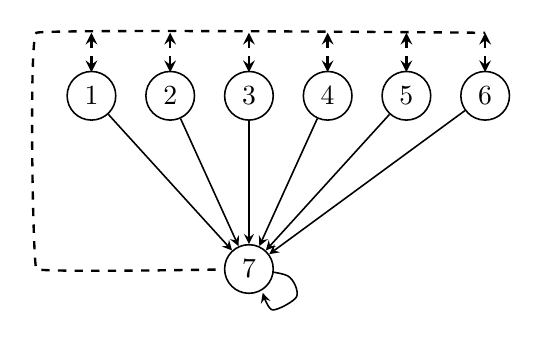
\begin{tikzpicture}[smooth]
\node[coordinate] (origin) at (0.3,0) {};
\node[coordinate] (num7) at (3,0) {};
\node[coordinate] (num1) at (1,2.5) {};
\path (num7) ++ (-10:0.5cm) node (num7_bright1) [coordinate] {};
\path (num7) ++ (-30:0.7cm) node (num7_bright2) [coordinate] {};
\path (num7) ++ (-60:0.35cm) node (num7_bright3) [coordinate] {};
\path (num7) ++ (-60:0.6cm) node (num7_bright4) [coordinate] {};
\path (origin) ++ (90:3cm) node (origin_above) [coordinate] {};
\path (origin_above) ++ (0:5.7cm) node (origin_aright) [coordinate] {};
\path (num1) ++ (90:0.5cm) node (num1_a) [coordinate] {};
\path (num1) ++ (-90:0.3cm) node (num1_b) [coordinate] {};

\path (num1) ++ (0:1cm) node (num2) [coordinate] {};
\path (num1_a) ++ (0:1cm) node (num2_a) [coordinate] {};
\path (num1_b) ++ (0:1cm) node (num2_b) [coordinate] {};
\path (num2) ++ (0:1cm) node (num3) [coordinate] {};
\path (num2_a) ++ (0:1cm) node (num3_a) [coordinate] {};
\path (num2_b) ++ (0:1cm) node (num3_b) [coordinate] {};
\path (num3) ++ (0:1cm) node (num4) [coordinate] {};
\path (num3_a) ++ (0:1cm) node (num4_a) [coordinate] {};
\path (num3_b) ++ (0:1cm) node (num4_b) [coordinate] {};
\path (num4) ++ (0:1cm) node (num5) [coordinate] {};
\path (num4_a) ++ (0:1cm) node (num5_a) [coordinate] {};
\path (num4_b) ++ (0:1cm) node (num5_b) [coordinate] {};
\path (num5) ++ (0:1cm) node (num6) [coordinate] {};
\path (num5_a) ++ (0:1cm) node (num6_a) [coordinate] {};
\path (num5_b) ++ (0:1cm) node (num6_b) [coordinate] {};


%\draw[->](0,0) -- (1,1);
%\draw[dashed,line width = 0.03cm] (0,0) -- (1,1);
 %\fill (0.5,0.5) circle (0.5);
 %\draw[shape=circle,fill=white,draw=black] (a) at (num7) {7};

 
\draw[dashed,line width = 0.03cm,xshift=3cm] plot[tension=0.06]
coordinates{(num7) (origin) (origin_above) (origin_aright)}; 

\draw[->,>=stealth,line width = 0.02cm,xshift=3cm] plot[tension=0.5]
coordinates{(num7) (num7_bright1) (num7_bright2)(num7_bright4) (num7_bright3)};
 
\node[line width = 0.02cm,shape=circle,fill=white,draw=black] (g) at (num7) {7};



\draw[<->,>=stealth,dashed,line width = 0.03cm,] (num1) -- (num1_a) ;
\node[line width = 0.02cm,shape=circle,fill=white,draw=black] (a) at (num1_b) {1};
\draw[<->,>=stealth,dashed,line width = 0.03cm,] (num2) -- (num2_a) ;
\node[line width = 0.02cm,shape=circle,fill=white,draw=black] (b) at (num2_b) {2};
\draw[<->,>=stealth,dashed,line width = 0.03cm,] (num3) -- (num3_a) ;
\node[line width = 0.02cm,shape=circle,fill=white,draw=black] (c) at (num3_b) {3};
\draw[<->,>=stealth,dashed,line width = 0.03cm,] (num4) -- (num4_a) ;
\node[line width = 0.02cm,shape=circle,fill=white,draw=black] (d) at (num4_b) {4};
\draw[<->,>=stealth,dashed,line width = 0.03cm,] (num5) -- (num5_a) ;
\node[line width = 0.02cm,shape=circle,fill=white,draw=black] (e) at (num5_b) {5};
\draw[<->,>=stealth,dashed,line width = 0.03cm,] (num6) -- (num6_a) ;
\node[line width = 0.02cm,shape=circle,fill=white,draw=black] (f) at (num6_b) {6};

\draw[->,>=stealth,line width = 0.02cm] (a)--(g);
\draw[->,>=stealth,line width = 0.02cm] (b)--(g);
\draw[->,>=stealth,line width = 0.02cm] (c)--(g);
\draw[->,>=stealth,line width = 0.02cm] (d)--(g);
\draw[->,>=stealth,line width = 0.02cm] (e)--(g);
\draw[->,>=stealth,line width = 0.02cm] (f)--(g);
\end{tikzpicture}
}


%         \label{7statebairdexample}
%     }
%         \caption{Three evaluation environments.}
%         \label{Threeevaluationenvironments}
%     \end{center}
%     \vskip -0.2in
% \end{figure*}
\subsection{Boychain}
\label{appendixboyanchian}
\textbf{Boyanchian:} BoyanChain is a classic on-policy environment 
with 13 states, each represented by a 4-dimensional feature vector. The agent 
can choose between two actions at each state: move to the next state (action 1) or skip to 
the one after (action 2). State 11 always transitions to state 12, while state 12 resets to 
state 0. Rewards are structured as follows: -2 for moving from state 11 to 12, 0 
for resetting from state 12 to 0, and -3 for all other actions. The policy is 
deterministic at state 11 (always choosing action 1) and stochastic elsewhere, 
randomly selecting between action 1 and 2. 
The discount factor $\gamma =0.9$. 
The feature matrix of Boyanchain is
defined as follows:
\begin{equation*}
    \bm{\Phi}_{Boyanchain}=\left[ 
    \begin{array}{cccc}
     1& 0& 0& 0\\
     0.75& 0.25& 0& 0\\
     0.5& 0.5& 0& 0\\
     0.25&0.75&0&0\\
     0& 1& 0& 0\\
     0& 0.75& 0.25& 0\\
    0 & 0.5& 0.5& 0\\
     0& 0.25& 0.75& 0\\
     0& 0& 1& 0\\
     0& 0& 0.75& 0.25\\
    0 & 0&0.5& 0.5\\
     0& 0& 0.25& 0.75\\
     0& 0& 0& 1
    \end{array}\right]
\end{equation*}
\begin{figure}[H]
    \begin{center}
    \label{boyanchianonpolicy}
    \includegraphics[width=0.5\columnwidth, height=0.2\columnwidth]{main/pic/boyanchian.png}
        \caption{Boychain.}
    \end{center}
\end{figure}
The $\alpha$ values for all algorithms are in the range of $\{0.0001, 0.0005, 0.001, 0.005, 0.01, 0.05, 0.1, 0.2, 0.3\}$. 
For the TDC and CTDC algorithm, the $\zeta$ values are in the range of $\{0.0005, 0.001, 0.005, 0.01, 0.05, 0.1, 0.2, 0.5\}$. 
For the CTD and CTDC algorithm, the $\beta$ values are in the range of $\{0.0005, 0.001, 0.005, 0.01, 0.05, 0.1, 0.2, 0.5\}$. 
\begin{figure}
    \vskip 0.2in
    \begin{center}
    \subfigure[TD]{
        \includegraphics[width=0.3\columnwidth, height=0.25\columnwidth]{main/pic/boyanchain/td/td.pdf}
        \label{td_boyanchain}
    }
    \subfigure[TDC]{
        \includegraphics[width=0.3\columnwidth, height=0.25\columnwidth]{main/pic/boyanchain/tdc/tdc.pdf}
        \label{tdc_boyanchain}
    }
    \subfigure[CTD]{
        \includegraphics[width=0.3\columnwidth, height=0.25\columnwidth]{main/pic/boyanchain/vmtd/vmtd.pdf}
        \label{ctd_boyanchain}
    }
    \\
    \subfigure[CTDC($\alpha=0.0001$)]{
        \includegraphics[width=0.3\columnwidth, height=0.25\columnwidth]{main/pic/boyanchain/vmtdc/alpha_0_0001.pdf}
        \label{ctdc_alpha_0001_boyanchain}
    }
    \subfigure[CTDC($\alpha=0.0005$)]{
        \includegraphics[width=0.3\columnwidth, height=0.25\columnwidth]{main/pic/boyanchain/vmtdc/alpha_0_0005.pdf}
        \label{ctdc_alpha_0005_boyanchain}
    }
    \subfigure[CTDC($\alpha=0.001$)]{
        \includegraphics[width=0.3\columnwidth, height=0.25\columnwidth]{main/pic/boyanchain/vmtdc/alpha_0_001.pdf}
        \label{ctdc_alpha_001_boyanchain}
    }
    \\
    \subfigure[CTDC($\alpha=0.005$)]{
        \includegraphics[width=0.3\columnwidth, height=0.25\columnwidth]{main/pic/boyanchain/vmtdc/alpha_0_005.pdf}
        \label{ctdc_alpha_005_boyanchain}
    }
    \subfigure[CTDC($\alpha=0.01$)]{
        \includegraphics[width=0.3\columnwidth, height=0.25\columnwidth]{main/pic/boyanchain/vmtdc/alpha_0_01.pdf}
        \label{ctdc_alpha_01_boyanchain}
    }
    \subfigure[CTDC($\alpha=0.05$)]{
        \includegraphics[width=0.3\columnwidth, height=0.25\columnwidth]{main/pic/boyanchain/vmtdc/alpha_0_05.pdf}
        \label{ctdc_alpha_05_boyanchain}
    }
    \\
    \subfigure[CTDC($\alpha=0.1$)]{
        \includegraphics[width=0.3\columnwidth, height=0.25\columnwidth]{main/pic/boyanchain/vmtdc/alpha_0_1.pdf}
        \label{ctdc_alpha_1_boyanchain}
    }
    \subfigure[CTDC($\alpha=0.2$)]{
        \includegraphics[width=0.3\columnwidth, height=0.25\columnwidth]{main/pic/boyanchain/vmtdc/alpha_0_2.pdf}
        \label{ctdc_alpha_2_boyanchain}
    }
    \subfigure[CTDC($\alpha=0.3$)]{
        \includegraphics[width=0.3\columnwidth, height=0.25\columnwidth]{main/pic/boyanchain/vmtdc/alpha_0_3.pdf}
        \label{ctdc_alpha_3_boyanchain}
    }
        \caption{Sensitivity of various algorithms to learning rates for Boyanchain.}
        \label{SensitivityBoyanchain}
    \end{center}
    \vskip -0.2in
\end{figure}
\subsection{2-state counterexample}
\label{appendix2state}
\textbf{2-state off-policy counterexample:} The ``1''$\rightarrow$``2'' problem has only two states \cite{sutton2016emphatic}. From each
state, there are two actions, left and right, which take 
the agent to the left or right state. All rewards are zero.
The feature $\bm{\Phi}=(1,2)^{\top}$ 
are assigned to the left and the right 
state. The behavior policy takes equal
probability to left or right
in both states, i.e., 
$
\textbf{P}_{1}=
\begin{bmatrix}
0.5 & 0.5 \\
0.5 & 0.5
\end{bmatrix}
$.
The target policy only selects action rights in both states, i.e., 
$
\textbf{P}_{2}=
\begin{bmatrix}
0 & 1 \\
0 & 1
\end{bmatrix}
$.
The state distribution of
the first policy is $\bm{d}_1 =(0.5,0.5)^{\top}$.
The state distribution of
the second policy is $\bm{d}_1 =(0,1)^{\top}$.
The discount factor is $\gamma=0.9$.
\begin{figure}[H]
    \begin{center}
    \label{bairdexampleoffpolicy}
    \includegraphics[width=0.3\columnwidth, height=0.1\columnwidth]{main/pic/2StateExample.pdf}
        \caption{2-state off-policy counterexample.}
    \end{center}
\end{figure}
The $\alpha$ values for all algorithms are in the range of $\{0.0001, 0.0005, 0.001, 0.005, 0.01\}$. 
For the TDC and CTDC algorithm, the $\zeta$ values are in the range of $\{0.0005, 0.001, 0.005, 0.01, 0.05\}$. 
For the CTD and CTDC algorithm, the $\beta$ values are in the range of $\{0.0005, 0.001, 0.005, 0.01, 0.05, 0.1, 0.2\}$. 
\begin{figure}
    \vskip 0.2in
    \begin{center}
    \subfigure[TD]{
        \includegraphics[width=0.3\columnwidth, height=0.25\columnwidth]{main/pic/2_state/td/td.pdf}
        \label{td_2state}
    }
    \subfigure[TDC]{
        \includegraphics[width=0.3\columnwidth, height=0.25\columnwidth]{main/pic/2_state/tdc/tdc.pdf}
        \label{tdc_2state}
    }
    \subfigure[CTD]{
        \includegraphics[width=0.3\columnwidth, height=0.25\columnwidth]{main/pic/2_state/ctd/ctd.pdf}
        \label{ctd_2state}
    }
    \\
    \subfigure[CTDC($\alpha=0.0001$)]{
        \includegraphics[width=0.3\columnwidth, height=0.25\columnwidth]{main/pic/2_state/ctdc/alpha_0_0001.pdf}
        \label{ctdc_alpha_0001_2state}
    }
    \subfigure[CTDC($\alpha=0.0005$)]{
        \includegraphics[width=0.3\columnwidth, height=0.25\columnwidth]{main/pic/2_state/ctdc/alpha_0_0005.pdf}
        \label{ctdc_alpha_0005_2state}
    }
    \subfigure[CTDC($\alpha=0.001$)]{
        \includegraphics[width=0.3\columnwidth, height=0.25\columnwidth]{main/pic/2_state/ctdc/alpha_0_001.pdf}
        \label{ctdc_alpha_001_2state}
    }
    \\
    \subfigure[CTDC($\alpha=0.005$)]{
        \includegraphics[width=0.3\columnwidth, height=0.25\columnwidth]{main/pic/2_state/ctdc/alpha_0_005.pdf}
        \label{ctdc_alpha_005_2state}
    }
    \subfigure[CTDC($\alpha=0.01$)]{
        \includegraphics[width=0.3\columnwidth, height=0.25\columnwidth]{main/pic/2_state/ctdc/alpha_0_01.pdf}
        \label{ctdc_alpha_01_2state}
    }
    \subfigure[CTDC($\alpha=0.05$)]{
        \includegraphics[width=0.3\columnwidth, height=0.25\columnwidth]{main/pic/2_state/ctdc/alpha_0_05.pdf}
        \label{ctdc_alpha_05_2staten}
    }
    \\
    \subfigure[CTDC($\alpha=0.1$)]{
        \includegraphics[width=0.3\columnwidth, height=0.25\columnwidth]{main/pic/2_state/ctdc/alpha_0_1.pdf}
        \label{ctdc_alpha_1_2state}
    }
    \subfigure[CTDC($\alpha=0.2$)]{
        \includegraphics[width=0.3\columnwidth, height=0.25\columnwidth]{main/pic/2_state/ctdc/alpha_0_2.pdf}
        \label{ctdc_alpha_2_2state}
    }
    \subfigure[CTDC($\alpha=0.3$)]{
        \includegraphics[width=0.3\columnwidth, height=0.25\columnwidth]{main/pic/2_state/ctdc/alpha_0_3.pdf}
        \label{ctdc_alpha_3_2staten}
    }
        \caption{Sensitivity of various algorithms to learning rates for 2-state counterexample.}
        \label{Sensitivity2state}
    \end{center}
    \vskip -0.2in
\end{figure}
\subsection{7-state counterexample}
\label{appendix7state}
\textbf{7-state off-policy counterexample:} This task is well known as a
counterexample, in which TD diverges \cite{baird1995residual,sutton2009fast}. As
shown in Figure \ref{7statebairdexample}, reward for each transition is zero. Thus the true values are zeros for all states and for any given policy. The behaviour policy
chooses actions represented by solid lines with a probability of $\frac{1}{7}$
and actions represented by dotted lines with a probability of $\frac{6}{7}$. The
target policy is expected to choose the solid line with more probability than $\frac{1}{7}$,
and it chooses the solid line with probability of $1$ in this paper.
 The discount factor $\gamma =0.99$. 
The feature matrix of 7-state version of Baird's off-policy counterexample is
defined as follows \ref{appendix7state} \cite{baird1995residual,sutton2009fast,maei2011gradient}:
\begin{equation*}
    \bm{\Phi}_{Counter}=\left[ 
\begin{array}{cccccccc}
1 & 2& 0& 0& 0& 0& 0& 0\\
1 & 0& 2& 0& 0& 0& 0& 0\\
1 & 0& 0& 2& 0& 0& 0& 0\\
1 & 0& 0& 0& 2& 0& 0& 0\\
1 & 0& 0& 0& 0& 2& 0& 0\\
1 & 0& 0& 0& 0& 0& 2& 0\\
2 & 0& 0& 0& 0& 0& 0& 1
\end{array}\right]
\end{equation*}
\begin{figure}[H]
    \begin{center}
        \resizebox{5cm}{3cm}{
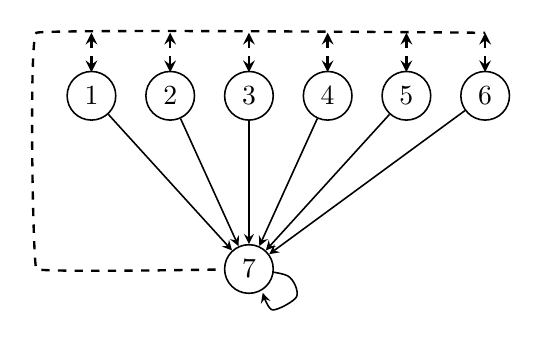
\begin{tikzpicture}[smooth]
\node[coordinate] (origin) at (0.3,0) {};
\node[coordinate] (num7) at (3,0) {};
\node[coordinate] (num1) at (1,2.5) {};
\path (num7) ++ (-10:0.5cm) node (num7_bright1) [coordinate] {};
\path (num7) ++ (-30:0.7cm) node (num7_bright2) [coordinate] {};
\path (num7) ++ (-60:0.35cm) node (num7_bright3) [coordinate] {};
\path (num7) ++ (-60:0.6cm) node (num7_bright4) [coordinate] {};
\path (origin) ++ (90:3cm) node (origin_above) [coordinate] {};
\path (origin_above) ++ (0:5.7cm) node (origin_aright) [coordinate] {};
\path (num1) ++ (90:0.5cm) node (num1_a) [coordinate] {};
\path (num1) ++ (-90:0.3cm) node (num1_b) [coordinate] {};

\path (num1) ++ (0:1cm) node (num2) [coordinate] {};
\path (num1_a) ++ (0:1cm) node (num2_a) [coordinate] {};
\path (num1_b) ++ (0:1cm) node (num2_b) [coordinate] {};
\path (num2) ++ (0:1cm) node (num3) [coordinate] {};
\path (num2_a) ++ (0:1cm) node (num3_a) [coordinate] {};
\path (num2_b) ++ (0:1cm) node (num3_b) [coordinate] {};
\path (num3) ++ (0:1cm) node (num4) [coordinate] {};
\path (num3_a) ++ (0:1cm) node (num4_a) [coordinate] {};
\path (num3_b) ++ (0:1cm) node (num4_b) [coordinate] {};
\path (num4) ++ (0:1cm) node (num5) [coordinate] {};
\path (num4_a) ++ (0:1cm) node (num5_a) [coordinate] {};
\path (num4_b) ++ (0:1cm) node (num5_b) [coordinate] {};
\path (num5) ++ (0:1cm) node (num6) [coordinate] {};
\path (num5_a) ++ (0:1cm) node (num6_a) [coordinate] {};
\path (num5_b) ++ (0:1cm) node (num6_b) [coordinate] {};


%\draw[->](0,0) -- (1,1);
%\draw[dashed,line width = 0.03cm] (0,0) -- (1,1);
 %\fill (0.5,0.5) circle (0.5);
 %\draw[shape=circle,fill=white,draw=black] (a) at (num7) {7};

 
\draw[dashed,line width = 0.03cm,xshift=3cm] plot[tension=0.06]
coordinates{(num7) (origin) (origin_above) (origin_aright)}; 

\draw[->,>=stealth,line width = 0.02cm,xshift=3cm] plot[tension=0.5]
coordinates{(num7) (num7_bright1) (num7_bright2)(num7_bright4) (num7_bright3)};
 
\node[line width = 0.02cm,shape=circle,fill=white,draw=black] (g) at (num7) {7};



\draw[<->,>=stealth,dashed,line width = 0.03cm,] (num1) -- (num1_a) ;
\node[line width = 0.02cm,shape=circle,fill=white,draw=black] (a) at (num1_b) {1};
\draw[<->,>=stealth,dashed,line width = 0.03cm,] (num2) -- (num2_a) ;
\node[line width = 0.02cm,shape=circle,fill=white,draw=black] (b) at (num2_b) {2};
\draw[<->,>=stealth,dashed,line width = 0.03cm,] (num3) -- (num3_a) ;
\node[line width = 0.02cm,shape=circle,fill=white,draw=black] (c) at (num3_b) {3};
\draw[<->,>=stealth,dashed,line width = 0.03cm,] (num4) -- (num4_a) ;
\node[line width = 0.02cm,shape=circle,fill=white,draw=black] (d) at (num4_b) {4};
\draw[<->,>=stealth,dashed,line width = 0.03cm,] (num5) -- (num5_a) ;
\node[line width = 0.02cm,shape=circle,fill=white,draw=black] (e) at (num5_b) {5};
\draw[<->,>=stealth,dashed,line width = 0.03cm,] (num6) -- (num6_a) ;
\node[line width = 0.02cm,shape=circle,fill=white,draw=black] (f) at (num6_b) {6};

\draw[->,>=stealth,line width = 0.02cm] (a)--(g);
\draw[->,>=stealth,line width = 0.02cm] (b)--(g);
\draw[->,>=stealth,line width = 0.02cm] (c)--(g);
\draw[->,>=stealth,line width = 0.02cm] (d)--(g);
\draw[->,>=stealth,line width = 0.02cm] (e)--(g);
\draw[->,>=stealth,line width = 0.02cm] (f)--(g);
\end{tikzpicture}
}


        \label{7statebairdexample}
        \caption{7-state off-policy counterexample.}
    \end{center}
\end{figure}
The $\alpha$ values for all algorithms are in the range of $\{0.0001, 0.0005, 0.001, 0.005, 0.01, 0.05, 0.1, 0.2, 0.3\}$. 
For the TDC and CTDC algorithm, the $\zeta$ values are in the range of $\{0.0005, 0.001, 0.005, 0.01, 0.05, 0.1, 0.2\}$. 
For the CTD and CTDC algorithm, the $\beta$ values are in the range of $\{0.0005, 0.001, 0.005, 0.01, 0.05, 0.1, 0.2\}$. 
\begin{figure}
    \vskip 0.2in
    \begin{center}
    \subfigure[TD]{
        \includegraphics[width=0.3\columnwidth, height=0.25\columnwidth]{main/pic/7_state/td/td.pdf}
        \label{td_7state}
    }
    \subfigure[TDC]{
        \includegraphics[width=0.3\columnwidth, height=0.25\columnwidth]{main/pic/7_state/tdc/tdc.pdf}
        \label{tdc_7state}
    }
    \subfigure[CTD]{
        \includegraphics[width=0.3\columnwidth, height=0.25\columnwidth]{main/pic/7_state/ctd/ctd.pdf}
        \label{ctd_7state}
    }
    \\
    \subfigure[CTDC($\alpha=0.0001$)]{
        \includegraphics[width=0.3\columnwidth, height=0.25\columnwidth]{main/pic/7_state/ctdc/alpha_0_0001.pdf}
        \label{ctdc_alpha_0001_7state}
    }
    \subfigure[CTDC($\alpha=0.0005$)]{
        \includegraphics[width=0.3\columnwidth, height=0.25\columnwidth]{main/pic/7_state/ctdc/alpha_0_0005.pdf}
        \label{ctdc_alpha_0005_7state}
    }
    \subfigure[CTDC($\alpha=0.001$)]{
        \includegraphics[width=0.3\columnwidth, height=0.25\columnwidth]{main/pic/7_state/ctdc/alpha_0_001.pdf}
        \label{ctdc_alpha_001_7state}
    }
    \\
    \subfigure[CTDC($\alpha=0.005$)]{
        \includegraphics[width=0.3\columnwidth, height=0.25\columnwidth]{main/pic/7_state/ctdc/alpha_0_005.pdf}
        \label{ctdc_alpha_005_7state}
    }
    \subfigure[CTDC($\alpha=0.01$)]{
        \includegraphics[width=0.3\columnwidth, height=0.25\columnwidth]{main/pic/7_state/ctdc/alpha_0_01.pdf}
        \label{ctdc_alpha_01_7state}
    }
        \caption{Sensitivity of various algorithms to learning rates for 7-state counterexample.}
        \label{Sensitivity7state}
    \end{center}
    \vskip -0.2in
\end{figure}


\end{document}


% This document was modified from the file originally made available by
% Pat Langley and Andrea Danyluk for ICML-2K. This version was created
% by Iain Murray in 2018, and modified by Alexandre Bouchard in
% 2019 and 2021 and by Csaba Szepesvari, Gang Niu and Sivan Sabato in 2022.
% Modified again in 2023 and 2024 by Sivan Sabato and Jonathan Scarlett.
% Previous contributors include Dan Roy, Lise Getoor and Tobias
% Scheffer, which was slightly modified from the 2010 version by
% Thorsten Joachims & Johannes Fuernkranz, slightly modified from the
% 2009 version by Kiri Wagstaff and Sam Roweis's 2008 version, which is
% slightly modified from Prasad Tadepalli's 2007 version which is a
% lightly changed version of the previous year's version by Andrew
% Moore, which was in turn edited from those of Kristian Kersting and
% Codrina Lauth. Alex Smola contributed to the algorithmic style files.
